\documentclass[11pt, twoside, pdftex]{article}

% This include all the settings that we should use for the document
\newcommand{\PDFTitle}{Using the ModelSim-Intel FPGA Simulator by Drawing Waveforms}
\newcommand{\commonPath}{../../../Common}
\newcommand{\datePublished}{Mar 2022}

\newcommand{\versnum}{21.1} %version number quartus/AMP
\newcommand{\quartusname}{Quartus\textsuperscript{\textregistered} Prime}	
\newcommand{\textBar}{For \quartusname{} \versnum{}}
\newcommand{\thisyear}{2022 } %for copyright
\newcommand{\company}{FPGAcademy.org}
\newcommand{\longteamname}{FPGAcademy.org}
\newcommand{\teamname}{FPGAcademy}
\newcommand{\website}{FPGAcademy.org}

\newcommand{\productAcronym}{AMP}
\newcommand{\productNameShort}{Monitor Program}

\newcommand{\productNameMedTM}{Monitor Program}
\newcommand{\productNameMed}{Monitor Program}

%\newcommand{\headerLogoFilePath}[1]{#1/FPGAcademy.png}



\setlength\topmargin{-0.25in}
\setlength\headheight{0in}
\setlength\headsep{0.35in}
\setlength\textheight{8.5in}
\setlength\textwidth{7in}
\setlength\oddsidemargin{-0.25in}
\setlength\evensidemargin{-0.25in}
\setlength\parindent{0.25in}
\setlength\parskip{0in} 

\pdfpagewidth 8.5in
\pdfpageheight 11in

% listings is a package that supports encapsulating source code in LaTeX conveniently

\usepackage{listings}
% add support for graphics
\usepackage{graphicx}
\usepackage[usenames, dvipsnames]{color}

\def\expandparam\lstinputlisting[#1]#2{\edef\tmp{\noexpand\lstinputlisting[#1]{#2}}\tmp}

\widowpenalty 10000
\clubpenalty 10000

%%%%%%%%%%%%%%%%%%%% Source Code Formatting %%%%%%%%%%%%%%%%%%%%
\definecolor{globalCommentColour}{rgb}{0.588,0.588,0.588}

%%%%%%%%%%%%%%%%%%%%%%%%%%%%%%%%%%%%%%%%%%%%%%%%%%%%
% Defining a NiosII ASM highlighter for lstlisting
\lstdefinelanguage[NiosII]{Assembler} {
 	morekeywords={add, addi, and, andhi, andi, beq, bge, bgeu, bgt, bgtu, ble,  bleu, blt, bltu, bne, br, break,% 
 	bret, call, callr, cmpeq, cmpeqi, cmpge, cmpgei, cmpgeu, cmpgeui, cmpgt, cmpgti, cmpgtu, cmpgtui, cmple,%
 	cmplei, cmpleu, cmpleui, cmplt, cmplti, cmpltu, cmpltui, cmpne, cmpnei, custom, div, divu, eret, flushd,%
 	flushda, flushi, flushp, initd, initda, initi, jmp, jmpi, ldb, ldbio, ldbu, ldbuio, ldh, ldhio, ldhu, ldhuio,%
 	ldw, ldwio, mov, movhi, movi, movia, movui, mul, muli, mulxss, mulxsu, mulxuu, nextpc, nop, nor, or, orhi, ori,%
 	rdctl, rdprs, ret, rol, roli, ror, sll, slli, sra, srai, srl, srli, stb, stbio, sth, sthio, stw, stwio,%
 	sub, subi, sync, trap, wrctl, wrtcl, wrprs, xor, xori, xorhi, xori},% 	
 	morekeywords=[2]{.abort, .ABORT, .align, .app-file, .ascii, .asciz, .balign, .byte, .comm, .data, .def,%
 	.desc, .dim, .double, .eject, .else, .end, .endef, .endif, .equ, .equiv, .err, .extern, .file, .fill, .float,%
 	.global, .globl, .hword, .ident, .if, .include, .int, .irp, .irpc, .lcomm, .lflags, .line, .linkonce, .ln,%
 	.list, .long, .macro, .mri, .nolist, .octa, .org, .p2align, .psize, .quad, .rept, .sbttl, .scl, .section,%
 	.set, .short, .single, .size, .sleb128, .skip, .space, .stadb, .stabn, .stabs, .string, .symver, .tag,%
 	.text, .title, .type, .val, .uleb128, .word},% 	
 	morekeywords=[3]{et, bt, gp, sp, fp, ea, sstatus, ra, pc, status, estatus, bstatus, ienable, ipending, cpuid,%
 	exception, pteaddr, tlbacc, tlbmisc, eccinj, badaddr, config, mpubase, mpuacc},% 	
 	sensitive=t,%
 	alsoletter=.,%
	morestring=[b]",%
 	morecomment=[s]{/*}{*/},%
 	morecomment=[l]\#,%
   }[keywords,comments,strings]
   
   %% NOTE: morekeywords=[2] are GNU directives.
   
   \definecolor{niosInstructionColour}{rgb}{0.000,0.608,0.000}
   \definecolor{niosDirectiveColour}{rgb}{0.000,0.000,0.902}
   \definecolor{niosSpecialRegColour}{rgb}{0.000,0.000,0.000}
   \definecolor{niosStringColour}{rgb}{0.808,0.482,0.000}
   
   %% NOTE: To make bold use: =\bfseries\color{<colour>}
   \lstdefinestyle{defaultNiosStyle} {
   language=[NiosII]{Assembler},
   stringstyle=\color{niosStringColour},
   keywordstyle=\color{niosInstructionColour},
   keywordstyle=[2]\color{niosDirectiveColour},
   keywordstyle=[3]\itshape\color{niosSpecialRegColour}
   }
%%%%%%%%%%%%%%%%%%%%%%%%%%%%%%%%%%%%%%%%%%%%%%%%%%%%

%%%%%%%%%%%%%%%%%%%%%%%%%%%%%%%%%%%%%%%%%%%%%%%%%%%%
% Defining a ArmA9 ASM highlighter for lstlisting
\lstdefinelanguage[ArmA9]{Assembler} {
 	morekeywords={ADC, ADD, ADDS, AND, ANDS, B, BAL, BEQ, BGE, BGT, BL, BLT, BIC, BKPT, BLX, BNE, BX, CDP, CLZ, CMN, CMP, EOR,%
 	EORS, LDC, LDM, LDR, LDRB, LDRBT, LDRH, LDRSB, LDRSH, LDRT, LSL, MCR, MLA, MOV, MOVW, MOVT, MRC, MRS, MSR, MUL, MVN, ORR, PLD,%
 	ROR, RSB, RSC, SBC, SMLAL, SMULL, STC, STM, STR, STRB, STRBT, STRH, STRT, SUB, SUBS, SWI, SWP, SWPB, TEQ, UMLAL,
 	PUSH, POP, MOVS, RORS, LSR},%
 	morekeywords=[2]{.abort, .ABORT, .align, .app-file, .ascii, .asciz, .balign, .byte, .comm, .data, .def,%
 	.desc, .dim, .double, .eject, .else, .end, .endef, .endif, .equ, .equiv, .err, .extern, .file, .fill, .float,%
 	.global, .globl, .hword, .ident, .if, .include, .int, .irp, .irpc, .lcomm, .lflags, .line, .linkonce, .ln,%
 	.list, .long, .macro, .mri, .nolist, .octa, .org, .p2align, .psize, .quad, .rept, .sbttl, .scl, .section,%
 	.set, .short, .single, .size, .sleb128, .skip, .space, .stadb, .stabn, .stabs, .string, .symver, .tag,%
 	.text, .title, .type, .val, .vectors, .uleb128, .word},%
 	morekeywords=[3]{SP, PC, MIDR, CTR, TCMTR, TLBTR, MPIDR, ID_PFR0, ID_PFR1, ID_DFR0, ID_MMFR0, ID_MMFR1, ID_MMFR2,%
 	ID_MMFR3, ID_ISAR0, ID_ISAR1, ID_ISAR2, ID_ISAR3, ID_ISAR4, CCSIDR, CLIDR, AIDR, CSSELR, TTBR0, TTRB1, TTBR2, DACR,%
 	DFSR, IFSR, ADFSR, AIFSR, DFAAR, IFAR, ICIALLUIS, BPIALLIS, PAR, ICIALLU, ICIMVAU, BPIALL, DCIMVAC, DCISW, V2PCWPR,%
 	DCCVAC, DCCSW, DDIMVAC, DCISW, TLBALLIS, TLBIMVAIS, TLBIASIDIS, TLBIMVAAIS, TLBIALL, TLBIMVA, TLBIASID, TLBIMVAA,%
 	PMCR, PMCNTENSET, PMCNTENCLR, PMOVSR, PMSWINC, PMSELR, PMXEVTYPER, PMXEVCNTR, PMUSERENR, PMINTENSET, PMINTENCLR,%
 	PRRR, NRRR, PLEIDR, PLEASR, PLEFSR, PLEUAR, PLEPCR, VBAR, MVBAR, ISR, FCSEIDR, CONTEXTIDR, TPIDRURW, TPIDRURO, TPIDRPRW},%
 	sensitive=f,%
 	alsoletter=.,%
	morestring=[b]",%
 	morecomment=[s]{/*}{*/},%
 	morecomment=[l]{//},%
   }[keywords,comments,strings]
   
   %% NOTE: morekeywords=[2] are GNU directives.
   
   \definecolor{armInstructionColour}{rgb}{0.000,0.608,0.000}
   \definecolor{armDirectiveColour}{rgb}{0.000,0.000,0.902}
   \definecolor{armSpecialRegColour}{rgb}{0.000,0.000,0.000}
   \definecolor{armStringColour}{rgb}{0.808,0.482,0.000}
   
   \lstdefinestyle{defaultArmStyle} {
   language=[ArmA9]{Assembler},
   stringstyle=\color{armStringColour},
   keywordstyle=\color{armInstructionColour},
   keywordstyle=[2]\color{armDirectiveColour},
   keywordstyle=[3]\itshape\color{armSpecialRegColour}
   }
%%%%%%%%%%%%%%%%%%%%%%%%%%%%%%%%%%%%%%%%%%%%%%%%%%%%

%%%%%%%%%%%%%%%%%%%%%%%%%%%%%%%%%%%%%%%%%%%%%%%%%%%%
% Defining style for the verilog.

\definecolor{verilogCommentColour}{rgb}{0.000,0.502,0.000}

\lstdefinestyle{defaultVerilogStyle} {
language={Verilog},
keywordstyle=\color{blue},
commentstyle=\color{verilogCommentColour}
}
%%%%%%%%%%%%%%%%%%%%%%%%%%%%%%%%%%%%%%%%%%%%%%%%%%%%

%%%%%%%%%%%%%%%%%%%%%%%%%%%%%%%%%%%%%%%%%%%%%%%%%%%%
% Defining style for the vhdl.
\lstdefinestyle{defaultVHDLStyle} {
language={VHDL},
keywordstyle=\color{blue},
commentstyle=\color{verilogCommentColour}
}
%%%%%%%%%%%%%%%%%%%%%%%%%%%%%%%%%%%%%%%%%%%%%%%%%%%%

%%%%%%%%%%%%%%%%%%%%%%%%%%%%%%%%%%%%%%%%%%%%%%%%%%%%
% Java
\definecolor{javaStringColour}{rgb}{0.808,0.482,0}
%%%%%%%%%%%%%%%%%%%%%%%%%%%%%%%%%%%%%%%%%%%%%%%%%%%%

%%%%%%%%%%%%%%%%%%%%%%%%%%%%%%%%%%%%%%%%%%%%%%%%%%%%
% Defining language styles
% C
\definecolor{CStringColour}{rgb}{0.808,0.482,0}
%%%%%%%%%%%%%%%%%%%%%%%%%%%%%%%%%%%%%%%%%%%%%%%%%%%%

%%%%%%%%%%%%%%%%%%%%%%%%%%%%%%%%%%%%%%%%%%%%%%%%%%%%
% Defining extended LaTeX language.
\lstdefinelanguage[LocalLaTeX]{TeX}[LaTeX]{TeX}%
 	{moretexcs={bf, it, sf, lstset},%
   	}%

\lstdefinestyle{defaultLocalLatexStyle} {
language=[LocalLatex]{TeX},
keywordstyle=\color{blue}\bfseries,
keywordstyle=[2]\color{blue},
keywordstyle=[3]\color{blue}\bfseries
}
%%%%%%%%%%%%%%%%%%%%%%%%%%%%%%%%%%%%%%%%%%%%%%%%%%%%

\lstset{
%language = C,
%language = Verilog,
%basicstyle=\color{black}\rmfamily\ttfamily,
basicstyle=\small\color{black}\ttfamily,
commentstyle=\small\color{globalCommentColour}\itshape\ttfamily,
keywordstyle=\small\color{blue}\bfseries\ttfamily,
showstringspaces=false,
frame=none, %lines % boxed listings
breaklines=true,
breakatwhitespace=true,
tabsize=4
}
%%%%%%%%%%%%%%%%%%%%%%%%%%%%%%%%%%%%%%%%%%%%%%%%%%%%%%%%%%%%%%%%


%\usepackage[centering]{geometry}.
%%%%%%%%%%%%%%%%%%%%%%%%%%%%%%%%%%%%%%%%%%%%%%%%%%%
% Document Settings
\usepackage[labelsep=period]{caption}
% we can choose a better font later
%\usepackage{palatino}
\usepackage{fourier}
%\fontencoding{T1}
% include common used symbols
\usepackage{textcomp}
% add support for graphics
\usepackage{graphicx}
\usepackage[usenames, dvipsnames]{color}
% enable to draw thick or thin table hlines
\setlength{\doublerulesep}{\arrayrulewidth}
\usepackage{longtable}
\setlongtables
%\usepackage{array}
% It may be better to use PDFLaTeX as it can generate bookmarks for the
% document

% Add some useful packages
\usepackage{ae,aecompl}
\usepackage{epsfig,float,times}

% reset the font for section
\usepackage{sectsty}
%\allsectionsfont{\fontfamily{ptm}\selectfont}
\allsectionsfont{\usefont{OT1}{phv}{bc}{n}\selectfont}

% use compact space for sections
\usepackage[compact]{titlesec}
\titlespacing{\section}{0pt}{0.2in}{*0}
\titlespacing{\subsection}{0pt}{0.1in}{*0}
\titlespacing{\subsubsection}{0pt}{0.05in}{*0}

% fancyhdr header and footer customization
\usepackage{layout}
\usepackage{fancyhdr}
\pagestyle{fancy}
\fancyhead{}
\fancyhead[R]{\textit{\tiny{\textBar}}}
\fancyfoot{}
\fancyfoot[LO,
RE]{\textrm{\href{https://www.fpgacademy.org}{\small \longteamname}} \\ {\small \datePublished }}
\fancyfoot[RO, LE]{\small \thepage}
% two-side settings
%\fancyhead{} % clear all header fields
%\fancyfoot{} % clear all footer fields
%\fancyfoot[LE,RO]{\thepage}
\renewcommand{\headrulewidth}{2pt}
\renewcommand{\headrule}{{\color{blue} \hrule width\headwidth height\headrulewidth \vskip-\headrulewidth}}
\renewcommand{\footrulewidth}{0pt}

% Format the footer on page 1
\fancypagestyle{plain}{
\fancyhead{}
\fancyfoot{}
\fancyfoot[LO,
RE]{\textrm{\href{https://www.fpgacademy.org}{\small \longteamname}} \\ {\small \datePublished }}
\fancyfoot[RO, LE]{\small \thepage}
\renewcommand{\headrulewidth}{0pt}
}
% adjust some setting to try to make the figure stay in the same page with text
% Reference: 	http://www.cs.uu.nl/~piet/floats/node1.html
%   			http://mintaka.sdsu.edu/GF/bibliog/latex/floats.html
%   General parameters, for ALL pages:
\renewcommand{\topfraction}{0.9}	% max fraction of floats at top
\renewcommand{\bottomfraction}{0.8}	% max fraction of floats at bottom
%   Parameters for TEXT pages (not float pages):
\setcounter{topnumber}{3}
\setcounter{bottomnumber}{3}
\setcounter{totalnumber}{5}     % 2 may work better
\setcounter{dbltopnumber}{2}    % for 2-column pages
\renewcommand{\dbltopfraction}{0.9}	% fit big float above 2-col. text
\renewcommand{\textfraction}{0.07}	% allow minimal text w. figs
%   Parameters for FLOAT pages (not text pages):
\renewcommand{\floatpagefraction}{0.7}	% require fuller float pages
% N.B.: floatpagefraction MUST be less than topfraction !!
\renewcommand{\dblfloatpagefraction}{0.7}	% require fuller float pages
%%%%%%%%%%%%%%%%%%%%%%%%%%%%%%%%%%%%%%%%%%%%%%%%%%%
% remember to use [htp] or [htpb] for placement
%%%%%%%%%%%%%%%%%%%%%%%%%%%%%%%%%%%%%%%%%%%%%%%%%%%

% set no indent for paragraph
\setlength{\parindent}{0em}
\addtolength{\parskip}{11pt}
\newcommand{\compact}{[topsep=0pt]}
% use this package to reduce space
\usepackage{enumitem}
\usepackage{multirow}
\usepackage{rotating}
\usepackage{pifont}
\usepackage{dingbat}
\newcommand{\itemsecond}{$\circ$}
%
%%%%%%%%%%%%%%%%%%
\date{}
\author{}
%%%%%%%%%%%%%%%%%%
\newcommand{\de}{DE-series}
\newcommand{\up}{FPGAcademy}
\newcommand{\fabric}{Avalon Switch Fabric}
\newcommand{\TODO}[1]{\textcolor{red}{\textbf{TODO}: #1}}
\def\registered{{\ooalign{\hfil\raise .00ex\hbox{\scriptsize R}\hfil\crcr\mathhexbox20D}}}

% enable url and reference(bookmarks) in pdf
\usepackage{url}
\usepackage[pdftex, colorlinks]{hyperref}
\hypersetup{%
pdftitle={\PDFTitle},
linkcolor=blue,
hyperindex=true,
pdfauthor={\longteamname},
pdfkeywords={FPGAcademy, Academic Program, Example System},
bookmarksnumbered,
bookmarksopen=false,
filecolor=blue,
pdfstartview={FitH},
urlcolor=blue,
plainpages=false,
pdfpagelabels=true,
linkbordercolor={1 1 1} %no color for link border
}%
%%%%%%%%%%%%%%%%%%%%%%%%%%%%%%%%%%%%%%%%%%%%%%%%%%%
\setlength{\fboxsep}{0.7pt}
\setlength{\fboxrule}{0.5pt}

\newcommand{\red}[1]{{\color{red}\sf{#1}}}
\newcommand{\blue}[1]{{\color{blue}\sf{#1}}}



%%%%%%%%%%%%%%%%%%%%%%%%%
% Add title
\newcommand{\doctitle}{Using the ModelSim-Intel FPGA \\ Simulator by Drawing Waveforms}
\newcommand{\dochead}{Using the ModelSim-Intel FPGA Simulator}
% Usually no need to change these two lines
\title{\fontfamily{phv}\selectfont{\doctitle} }
\chead{ \small{\textsc{\bfseries \dochead} } }
% Customizations
%%%%%%%%%%%%%%%%%%%%%%%%%
% Allows multiple figures per page

\renewcommand\floatpagefraction{.9}
\renewcommand\topfraction{.9}
\renewcommand\bottomfraction{.9}
\renewcommand\textfraction{.1}   
\setcounter{totalnumber}{50}
\setcounter{topnumber}{50}
\setcounter{bottomnumber}{50}
\raggedbottom

%%%%%%%%%%%%%%%%%%
%%% DOCUMENT START
%\begin{document}
\begin{document}
\begin{table}
    \centering
    \begin{tabular}{p{5cm}p{4cm}}
        \hspace{-3cm}
        &
        \raisebox{1\height}{\parbox[h]{0.5\textwidth}{\Large\fontfamily{phv}\selectfont{\textsf{\doctitle}}}}
    \end{tabular}
    \label{tab:logo}
\end{table}

\colorbox[rgb]{0,0.384,0.816}{\parbox[h]{\textwidth}{\color{white}\textsf{\textit{\textBar}}}}

\thispagestyle{plain}
 
\section{Introduction}

This tutorial introduces the simulation of Verilog code using the Graphical Waveform Editor
in the {\it ModelSim-Intel FPGA} simulator. We assume that you are using 
{\it ModelSim-Intel FPGA Starter Edition version 18.0}. This software can 
be downloaded and installed from the {\it Download Center for Intel FPGAs}. In this
download center, you can select release {\it 18.0} of the {\it Quartus Prime Lite Edition}, 
and then on the \texttt{Individual Files} tab choose to download and install the 
{\it ModelSim-Intel FPGA Starter Edition} software. We assume that you are using a computer
that is running the Windows operating system. If you are using the Linux operating system 
then minor differences to the instructions would apply, such as using a / filesystem delimiter 
rather than the $\backslash$ delimiter that is used with Windows. 

This tutorial is intended for introductory use of ModelSim by students who are just
beginning to learn about the relevant topics. For students who have gained some
familiarity with logic design and Verilog code we recommend the approach presented in the tutorial
{\it Using the ModelSim-Intel FPGA Simulator with Verilog Testbenches}.

{\bf Contents}:
\begin{itemize}
\item Design Project
\item Creating Waveforms for Simulation
\item Simulation
\item Making Changes and restarting the simulation
\end{itemize}

{\bf Requirements:}
\begin{itemize}
\item ModelSim-Intel FPGA Starter Edition software
\item A computer running either Microsoft* Windows* (version 10 is recommended) or Linux 
(Ubuntu, or a similar Linux distribution). The computer would typically be either a
desktop computer or laptop, and is used to run the ModelSim software.
\end{itemize}

{\bf Optional:}
\begin{itemize}
\item Intel Quartus\textsuperscript{\textregistered} Prime software
\item A DE-series development and education board, such as the DE1-SoC board. These boards are 
described on Intel's FPGA University Program website, and are available from the manufacturer 
Terasic Technologies.
\end{itemize}
\clearpage
\newpage
\section{Getting Started}

The ModelSim Simulator is a sophisticated and powerful tool that supports a variety of 
usage models. In this tutorial we focus on only one design flow: using the ModelSim
software as a {\it stand-alone} program to perform {\it functional} simulations, with 
simulation inputs specified by {\it drawing waveforms}, and with simulator commands selected 
by using the {\it menu items} that are available in ModelSim's graphical user interface
(GUI).  Other possible design flows for using ModelSim include {\it invoking} it from within the 
Intel Quartus Prime software, performing {\it timing} simulations, specifying simulation 
inputs by using a {\it testbench}, and selecting simulator commands via {\it script} files.
These flows are not described here, but can be found in other
documentation that is available on the Internet.  

This tutorial is aimed at the reader who wishes to simulate circuits defined
by using the Verilog hardware description language. An equivalent tutorial is
available for the user who prefers the VHDL language.
 
\section{Design Project}
When using the ModelSim GUI to execute simulation commands, it is convenient to work in the
context of a ModelSim {\it project}. A project includes the design files that specify the 
circuit to be simulated. We will first create a folder to hold the project used 
in this tutorial.  Create a new folder for this tutorial with a name such as
{\it ModelSim\_Tutorial} and then make a subfolder named {\it Majority} for this 
example project.

To illustrate the simulation process, we will use a very simple logic circuit that 
implements the majority function of three inputs, $x_1$, $x_2$ and $x_3$. The circuit
is defined by the expression
$$
f(x_1, x_2, x_3) = x_1 x_2 + x_1 x_3 + x_2 x_3
$$
\noindent
In Verilog, this circuit can be specified as follows:
~\\
\begin{lstlisting}[language=Verilog]
module majority (x1, x2, x3, f);
    input x1, x2, x3;
    output f;

    assign f = (x1 & x2) | (x1 & x3) | (x2 & x3);
endmodule
\end{lstlisting}
\noindent
Enter this code into a file called {\it majority.v}, in the folder 
{\it ModelSim\_Tutorial$\backslash$Majority}.
You can create the file using any text 
editor of your choosing (a text editor is also available within the ModelSim GUI).

Open the ModelSim simulator. In the displayed window select {\sf File $>$ New $>$ Project},
as shown in Figure~\ref{fig:1}.
A \texttt{Create Project} pop-up box will appear, as illustrated in Figure~\ref{fig:2}. 
Specify the name of the project; we chose the name {\it majority}. 
Use the {\sf Browse} button in the \texttt{Project Location} box to specify the location
of the folder that you created for the project.
ModelSim uses a working library to contain the information on the design 
in progress; in the \texttt{Default Library Name} field we used the name {\it work}.
Click {\sf OK}.

\begin{figure}[H]
   \begin{center}
      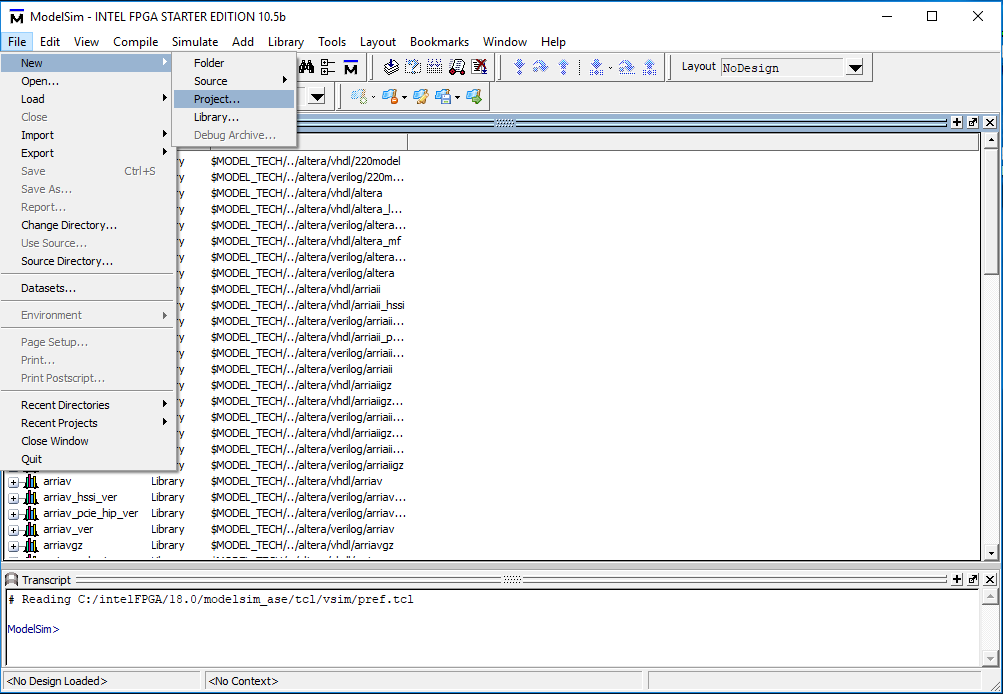
\includegraphics[scale=0.65]{figures/figure1.png}
   \caption{The ModelSim window.} 
	 \label{fig:1}
	 \end{center}
\end{figure}

\begin{figure}[H]
   \begin{center}
      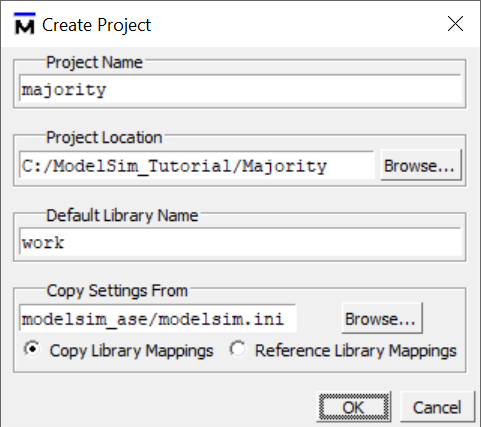
\includegraphics[scale=1.0]{figures/figure2.png}
   \caption{Created Project window.} 
	 \label{fig:2}
	 \end{center}
\end{figure}
\newpage
In the pop-up window in Figure~\ref{fig:3}, click on {\sf Add Existing File} and add the 
file {\it majority.v} to the project as shown in Figure~\ref{fig:4}. Click OK, then close the 
window from Figure~\ref{fig:3}.

\begin{figure}[H]
   \begin{center}
      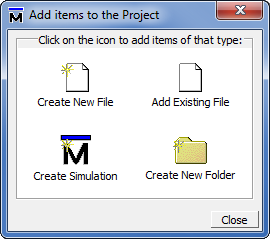
\includegraphics[scale=0.85]{figures/figure3.png}
   \caption{Add Items window.} 
	 \label{fig:3}
	 \end{center}
\end{figure}

\begin{figure}[H]
   \begin{center}
      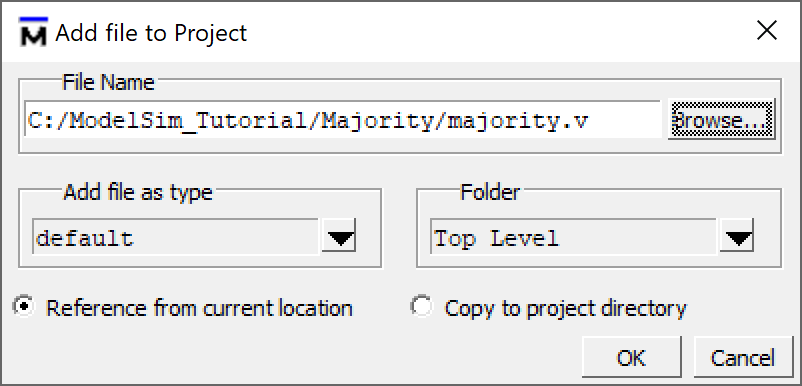
\includegraphics[scale=0.75]{figures/add_file.png}
   \caption{Add File window.} 
	 \label{fig:4}
	 \end{center}
\end{figure}

At this point, the main Modelsim window will include the file as indicated in 
Figure~\ref{fig:6}, with a question mark in the \texttt{Status} column. Now, select
{\sf Compile $>$ Compile All}. As illustrated in the figure, the ModelSim GUI will
indicate in the \texttt{Transcript} window (at the bottom) that the code in the {\it majority.v}
file was successfully compiled, and a corresponding check mark will be displayed in 
the \texttt{Status} column.  The Verilog code is now ready for simulation.

\begin{figure}[H]
   \begin{center}
      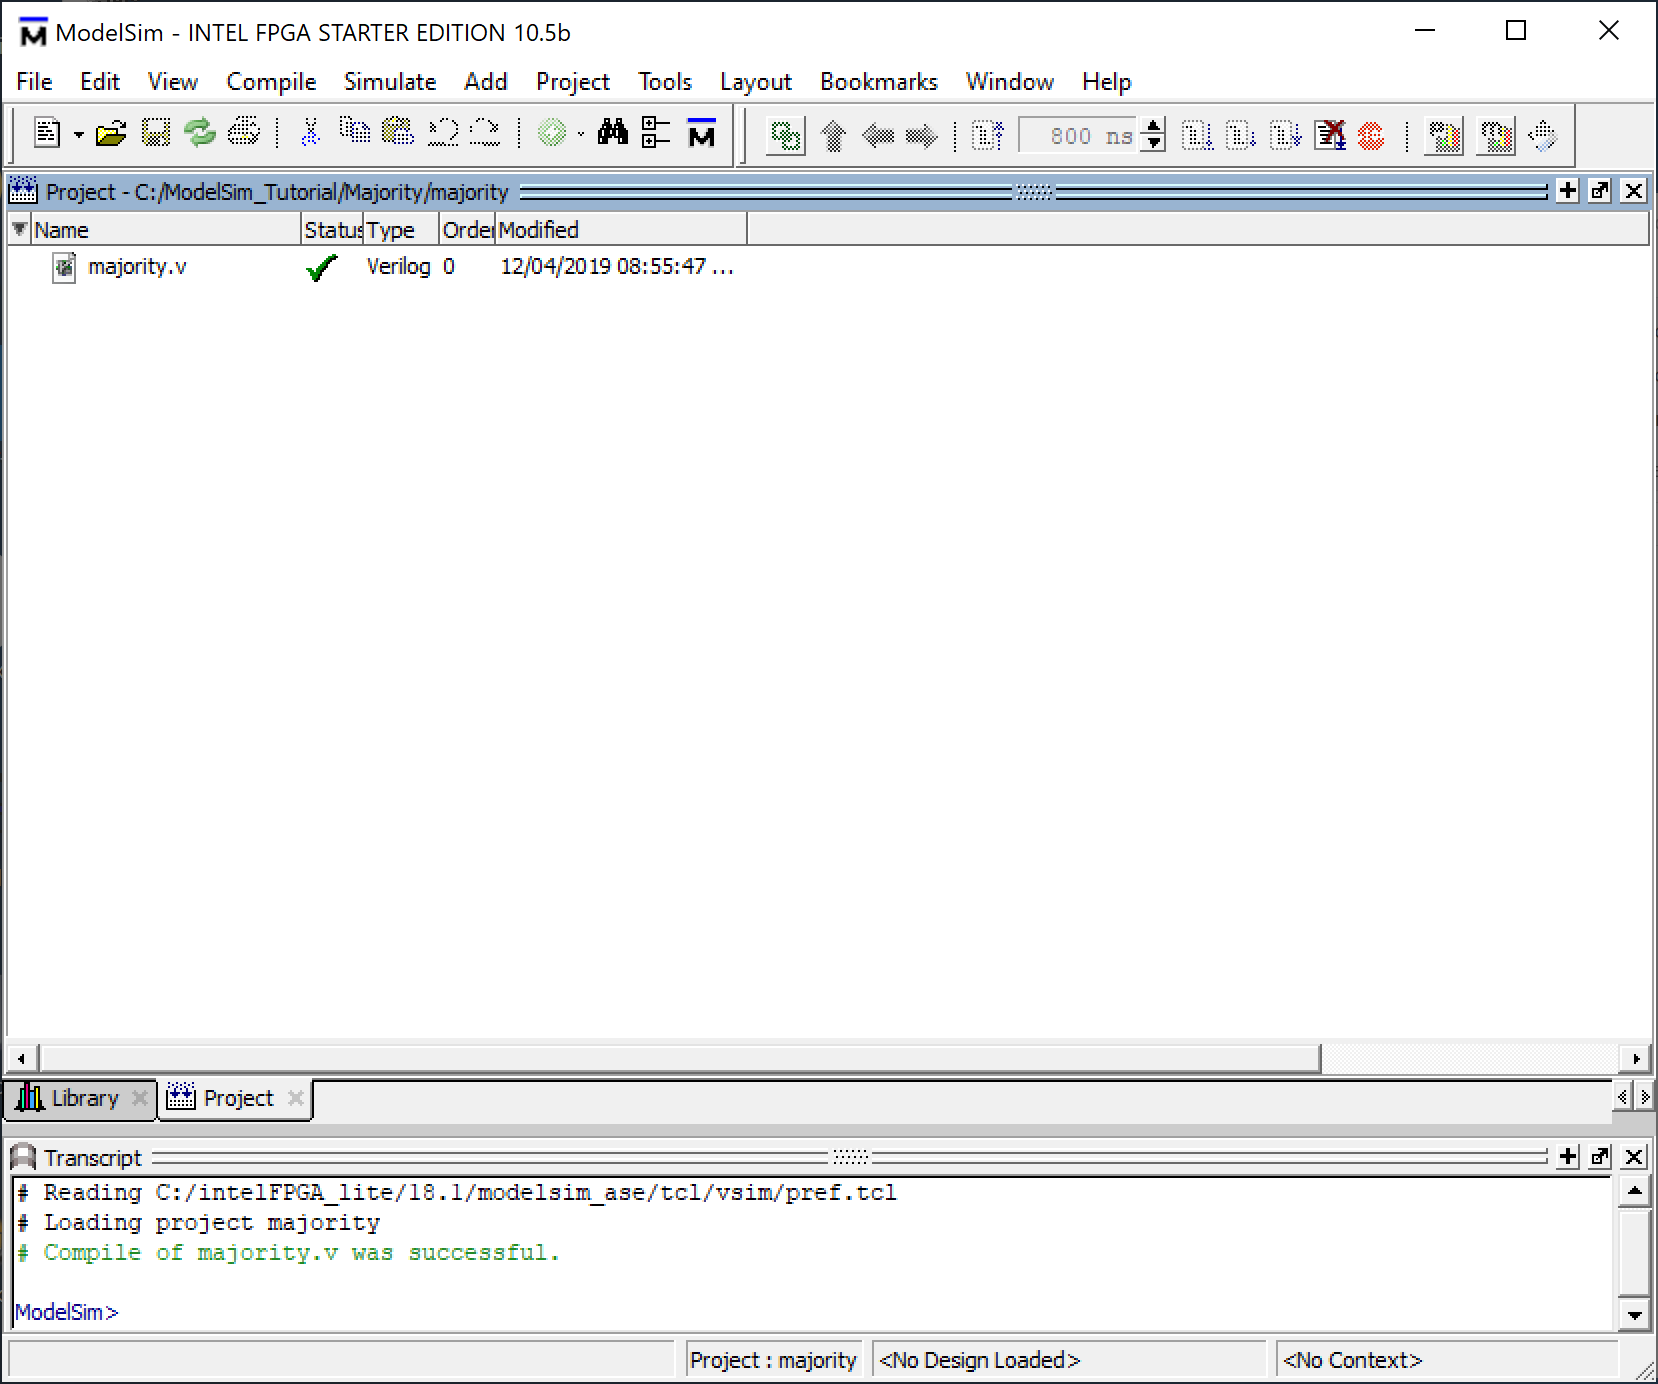
\includegraphics[scale=0.75]{figures/compile.png}
   \caption{ModelSim window after compilation.} 
	 \label{fig:6}
	 \end{center}
\end{figure}

\section{Creating Waveforms for Simulation}

To perform simulation of the designed circuit, it is necessary to enter the simulation mode
by selecting {\sf Simulate $>$ Start Simulation}. This leads to the window in Figure~\ref{fig:7}.

\begin{figure}[H]
   \begin{center}
      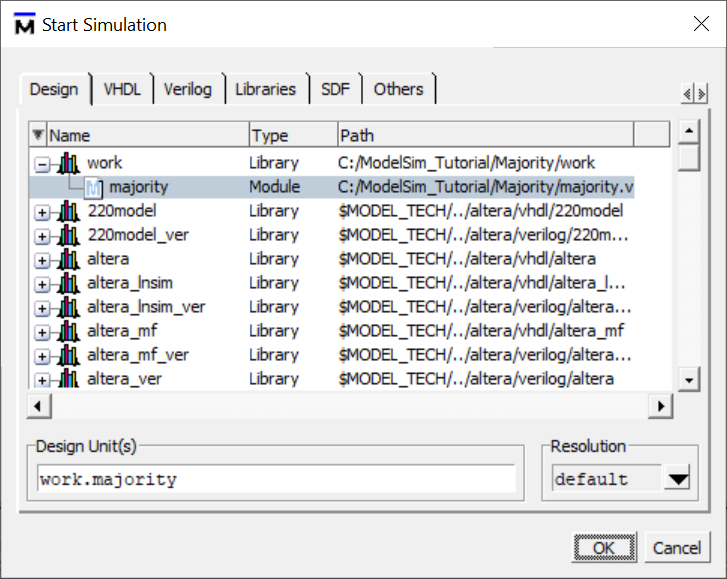
\includegraphics[scale=1.0]{figures/figure7.png}
   \caption{Start Simulation window.} 
	 \label{fig:7}
	 \end{center}
\end{figure}

Expand the {\it work} folder and select the design called {\it majority}, as shown in the
figure. Then click {\sf OK}. Now, the ModelSim GUI opens a number of windows and toolbars, 
as illustrated in Figure~\ref{fig:8}, that are useful for performing a simulation.  
The \texttt{Objects} window, shown in a blue color, lists the input and output signals 
of the designed circuit. The \texttt{Wave} window is used to display waveforms that are
associated with these inputs and outputs. Figure~\ref{fig:8} shows several toolbars 
that can be used to select various ModelSim GUI commands. To make your window look like 
the one in the figure, you may have to open or close some of the available toolbars. 
{\sf Right-clicking} in the toolbar area, as indicated in Figure~\ref{fig:toolbars}, 
allows you to show or hide toolbars.

\begin{figure}[H]
   \begin{center}
      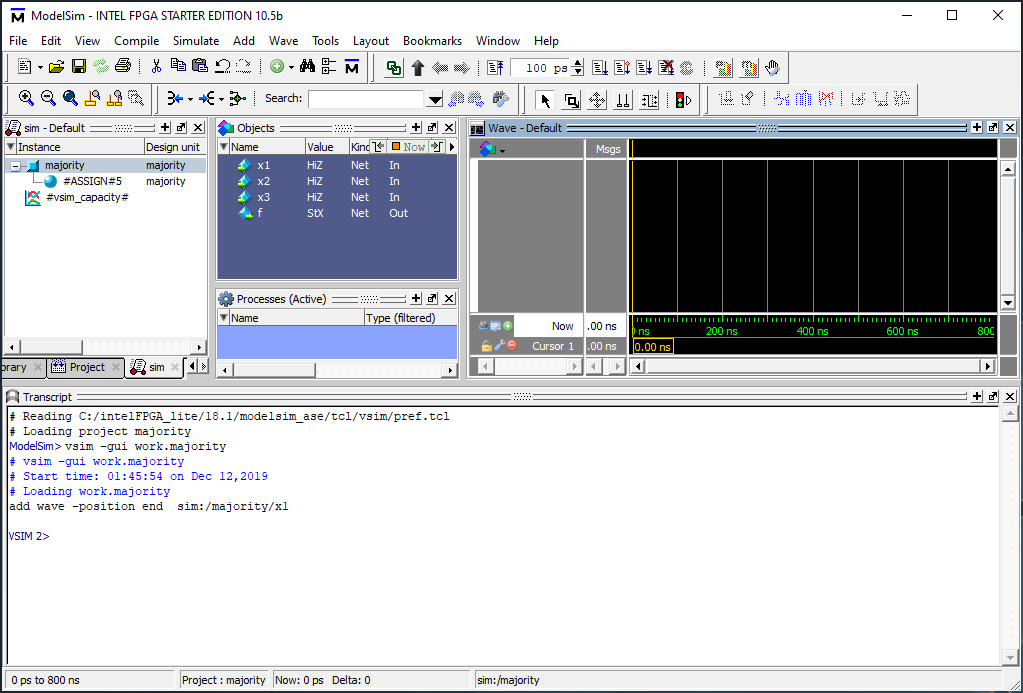
\includegraphics[width=\textwidth]{figures/sim_mode.png}
   \caption{Simulation windows.} 
	 \label{fig:8}
	 \end{center}
\end{figure}

\begin{figure}[H]
   \begin{center}
      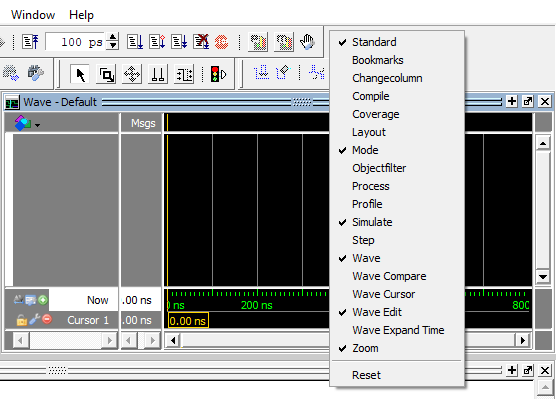
\includegraphics[scale=1.50]{figures/toolbar.png}
       \caption{The toolbars shown in Figure \ref{fig:8}.} 
	 \label{fig:toolbars}
	 \end{center}
\end{figure}

To simulate the circuit we must first specify the values of input signals, which can be done 
by drawing the input waveforms using the \texttt{Wave} window. Right-click in the \texttt{Wave}
window to select {\sf Zoom Range} and in the pop-up window that will appear specify the range 
from 0 to 800 ns. This selection should produce an image like the one in Figure~\ref{fig:9}.
If you need to change the timeline display units, right-click on the timeline and select 
{\sf Grid, Timeline, \& Cursor Control}, then select 
{\sf ns} in the \texttt{time units} drop-down menu.

\begin{figure}[H]
   \begin{center}
      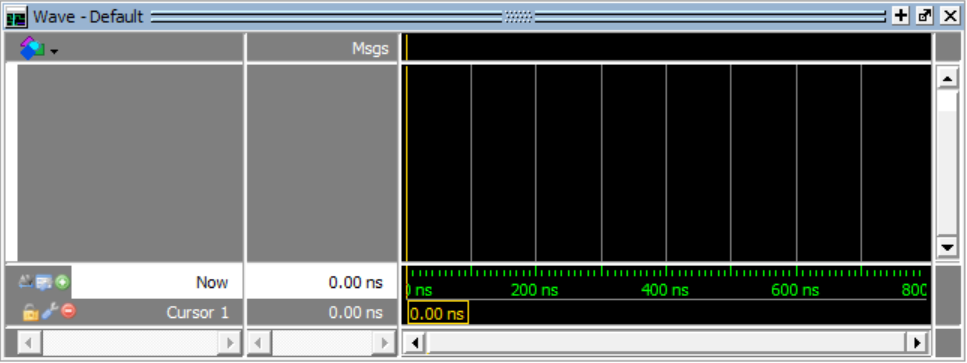
\includegraphics[scale=1.0]{figures/figure9.png}
       \caption{The \texttt{Wave} window.} 
	 \label{fig:9}
	 \end{center}
\end{figure}

For our simple circuit, we can do a complete simulation by applying all eight possible 
valuations of the input signals $x_1$, $x_2$ and $x_3$. The output $f$ should then display 
the logic values defined by the truth table for the majority function. We will first draw 
the waveform for the $x_1$ input.  In the \texttt{Objects} window, right-click on $x1$. Then, 
choose {\sf Modify $>$ Apply Wave} in the drop-down box that appears, as shown in 
Figure~\ref{fig:10}. This leads to the window in Figure~\ref{fig:11}, which makes it possible 
to specify the value of the selected signal in a time period that has to be defined. 
Choose {\sf Constant} as the desired pattern, zero as the start time, and 400 ns as 
the end time. Click {\sf Next}. In the window in Figure~\ref{fig:12}, enter 0 as the 
desired logic value. Click {\sf Finish}.  Now, the specified signal appears in the \texttt{Wave} 
window, as indicated in Figure~\ref{fig:13}.

\begin{figure}[H]
   \begin{center}
      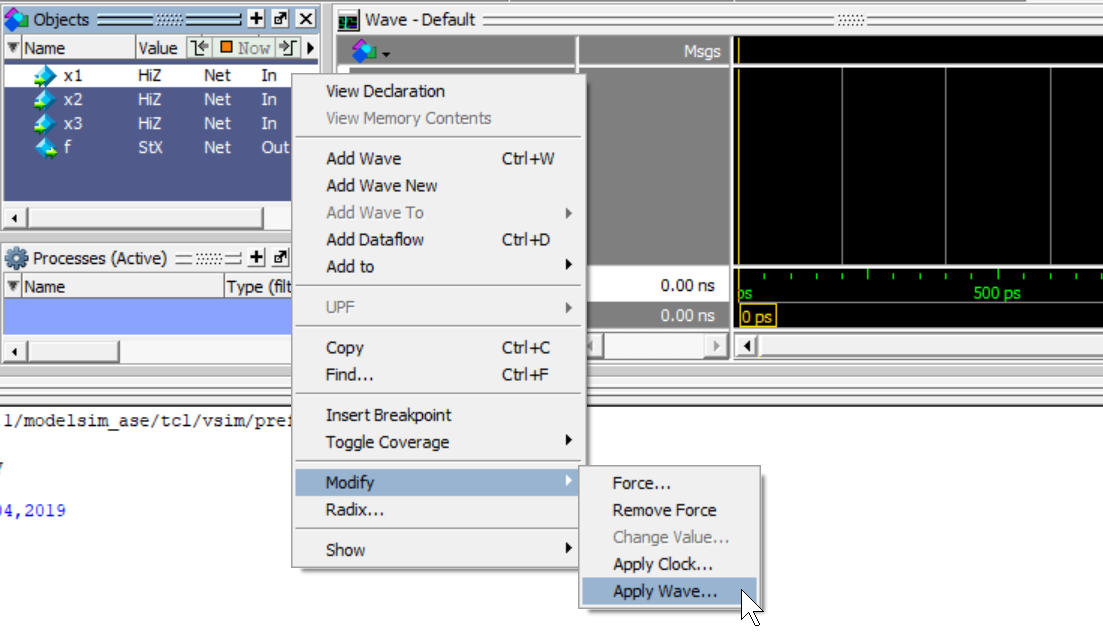
\includegraphics[scale=1.0]{figures/figure10.png}
       \caption{Selecting a signal in the \texttt{Objects} window.} 
	 \label{fig:10}
	 \end{center}
\end{figure}

\begin{figure}[H]
   \begin{center}
      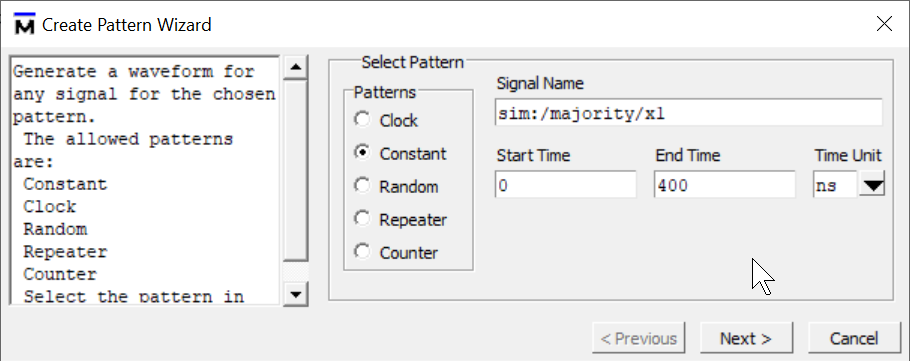
\includegraphics[scale=1.0]{figures/figure11.png}
   \caption{Specifying the type and duration of a signal.} 
	 \label{fig:11}
	 \end{center}
\end{figure}

\begin{figure}[H]
   \begin{center}
      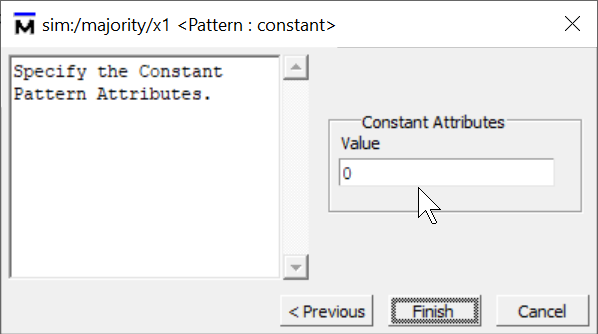
\includegraphics[scale=1.0]{figures/figure12.png}
   \caption{Specifying the value of a signal.} 
	 \label{fig:12}
	 \end{center}
\end{figure}

\begin{figure}[H]
   \begin{center}
      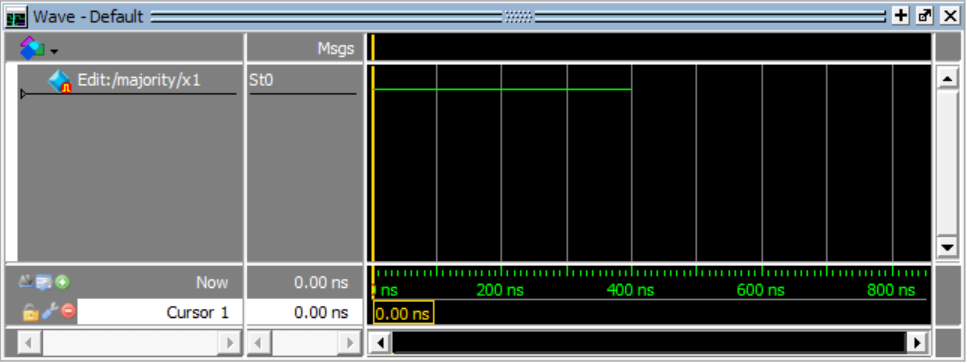
\includegraphics[scale=1.0]{figures/figure13.png}
       \caption{The updated \texttt{Wave} window.} 
	 \label{fig:13}
	 \end{center}
\end{figure}

To draw the rest of the $x_1$ signal, right-click on its name in the \texttt{Wave} window (make
sure to click in the \texttt{Wave} window to make this 
change to the existing waveform, and not in the \texttt{Objects} window).
In the drop-down window that appears, select {\sf Edit > Wave Editor > Create/Modify Waveform}.
This leads again to the window in Figure~\ref{fig:11}. Now, specify 400 ns as the start time
and 800 ns as the end time. Click {\sf Next}. In the window in Figure~\ref{fig:12}, specify
1 as the required logic value. Click {\sf Finish}. This completes the waveform for $x_1$,
as displayed in Figure~\ref{fig:14}.


\begin{figure}[H]
   \begin{center}
      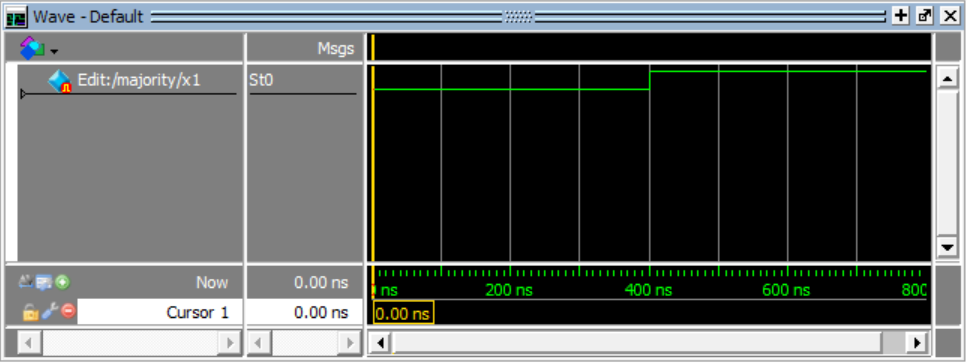
\includegraphics[scale=1.0]{figures/figure14.png}
   \caption{The completed waveform for $x_1$ input.} 
	 \label{fig:14}
	 \end{center}
\end{figure}

ModelSim provides different possibilities for creating and editing waveforms. To illustrate another
approach, we will specify the waveform for $x_2$ by first creating it to have a 0 value
throughout the simulation period, and then editing it to produce the required waveform.
Repeat the above procedure, by right-clicking on $x2$ in the \texttt{Objects} window,
to create a waveform for $x_2$ that has the value 0 in the interval 0 ns to 800 ns. 
So far, we used the \texttt{Wave} window in the \texttt{Select Mode} which is indicated by the 
highlighted icon  
\includegraphics[scale=1]{figures/icon2.png}. Now, click on the {\sf Edit Mode}
icon 
\includegraphics[scale=1]{figures/icon3.png} as indicated in Figure~\ref{fig:15} 
(if the \texttt{Edit Mode} icon is {\it greyed-out}, then first click on the title bar of the 
\texttt{Wave} window to activate it).  Note that \texttt{Edit Mode} opens some new toolbar 
icons for use in the editing process.

\begin{figure}[H]
   \begin{center}
      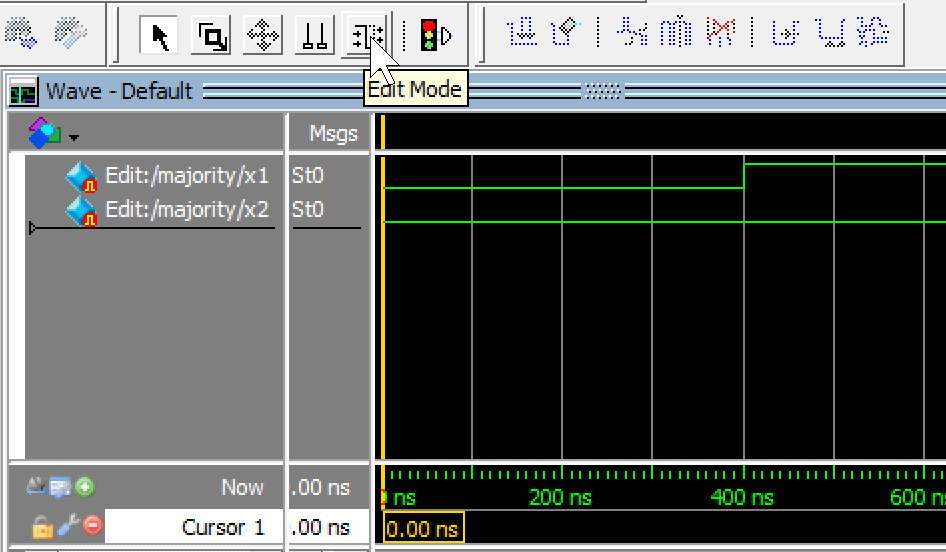
\includegraphics[scale=0.75]{figures/edit_mode.png}
   \caption{Selecting the Wave Edit mode.} 
	 \label{fig:15}
	 \end{center}
\end{figure}

The waveform for $x_2$ should change from 0 to 1 at 200 ns, then back to 0 at 400 ns, 
and again to 1 at 600 ns. Select $x2$ for editing by clicking on it. Then, click just to the 
right of the 200-ns point, hold the mouse button down and sweep to the right until 
you reach the 400-ns point. The chosen interval will be highlighted in white, as shown in 
Figure~\ref{fig:16}.  Observe that the yellow cursor line appears and moves as you sweep
along the time interval.  To change the value of the waveform in the selected interval, click on the 
{\sf Invert} icon as illustrated in the figure. A pop-up box in Figure~\ref{fig:17} will 
appear, showing the start and end times of the selected interval. If the displayed times are 
not exactly 200 and 400 ns, then correct them accordingly and click {\sf OK}. The modified 
waveform is displayed in Figure~\ref{fig:18}.  Use the same approach to change the value 
of $x_2$ to 1 in the interval from 600 to 800 ns, which should yield the result in 
Figure~\ref{fig:19}.

\begin{figure}[H]
   \begin{center}
      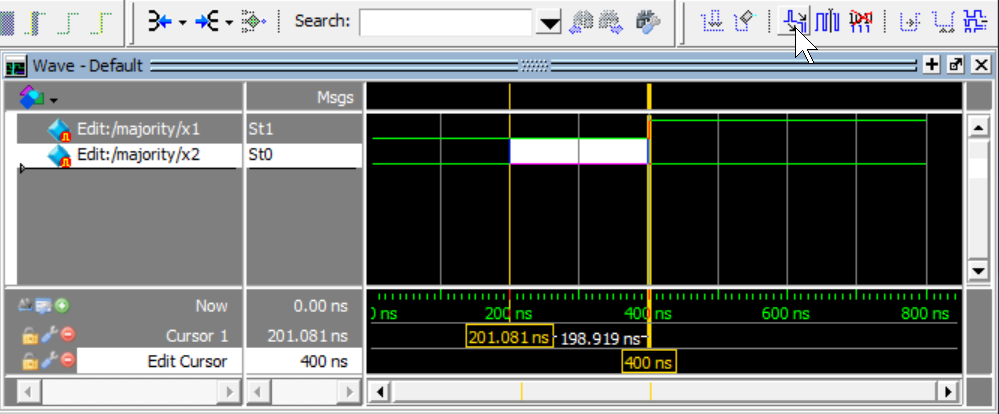
\includegraphics[scale=1.0]{figures/figure16.png}
   \caption{Editing the waveform.} 
	 \label{fig:16}
	 \end{center}
\end{figure}

\begin{figure}[H]
   \begin{center}
      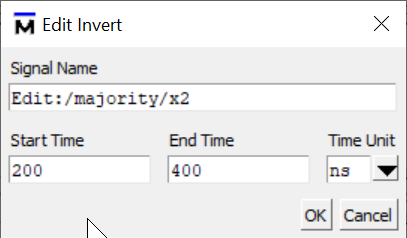
\includegraphics[scale=1.0]{figures/figure17.png}
   \caption{Specifying the exact time interval.} 
	 \label{fig:17}
	 \end{center}
\end{figure}

\begin{figure}[H]
   \begin{center}
      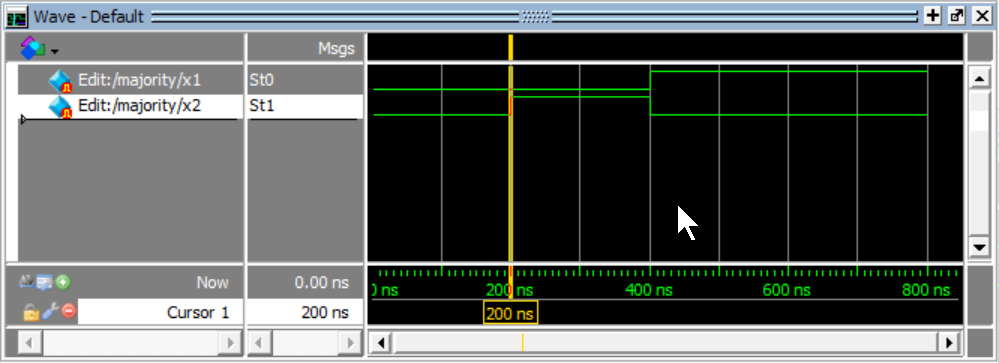
\includegraphics[scale=1.0]{figures/figure18.png}
   \caption{The modified waveform.} 
	 \label{fig:18}
	 \end{center}
\end{figure}

\begin{figure}[H]
   \begin{center}
      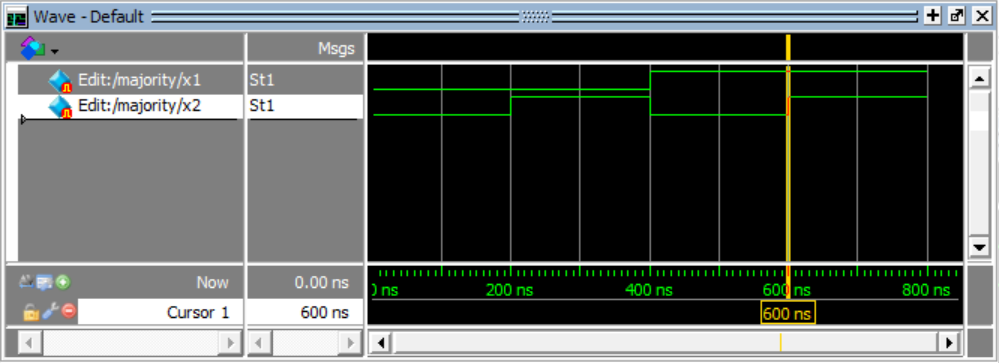
\includegraphics[scale=1.0]{figures/figure19.png}
   \caption{Completed waveforms for $x_1$ and $x_2$.} 
	 \label{fig:19}
	 \end{center}
\end{figure}

We will use a third approach to draw the waveform for $x_3$. This signal
should alternate between 0 and 1 logic values at each 100-ns interval.
Such a regular pattern is indicative of a {\it clock} signal that is used in many logic circuits.
To illustrate how a clock signal can be defined, we will specify $x_3$ in this manner.
Right-click on the $x_3$ input in the \texttt{Objects} window 
and select {\sf Modify $>$ Apply Wave}. 
In the \texttt{Create Pattern Wizard} window, select {\sf Clock} 
as the required pattern, and specify 
0 and 800 ns as the start and end times, respectively, as indicated in Figure~\ref{fig:20}.
Click {\sf Next}, which leads to the window in Figure~\ref{fig:21}. Here, specify 0 as the 
initial value, 200 ns as the clock period, and 50 as the duty cycle. Click {\sf Finish}.
Now, the waveform for $x_3$ is included in the \texttt{Wave} window.

\begin{figure}[H]
   \begin{center}
      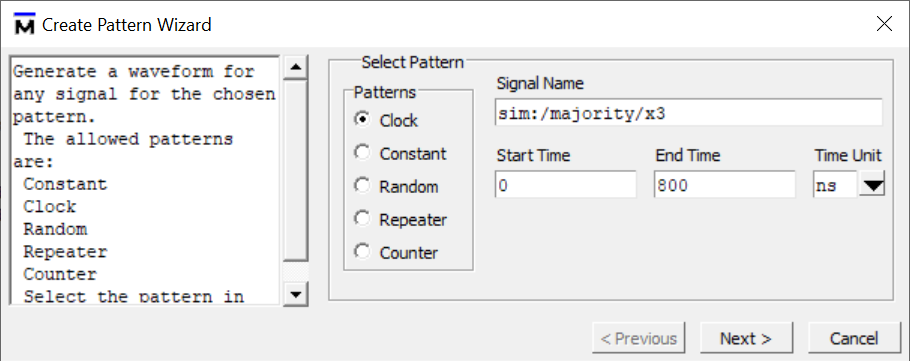
\includegraphics[scale=1.0]{figures/figure20.png}
   \caption{Selecting a signal of clock type.} 
	 \label{fig:20}
	 \end{center}
\end{figure}

\begin{figure}[H]
   \begin{center}
      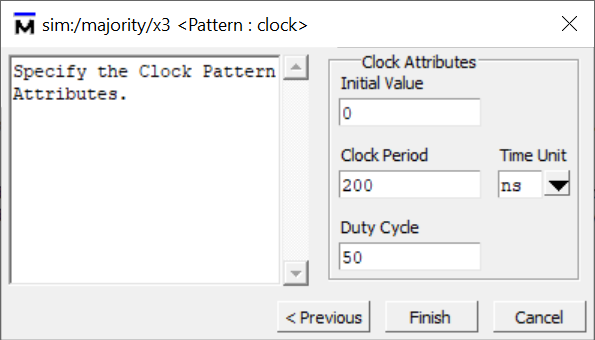
\includegraphics[scale=1.0]{figures/figure21.png}
   \caption{Defining the characteristics of a clock signal.} 
	 \label{fig:21}
	 \end{center}
\end{figure}

Lastly, it is necessary to include the output signal $f$. Right-click on $f$ in the
\texttt{Objects} window. In the drop-down menu that appears, select
{\sf Add to $>$ Wave $>$ Selected Signals} as shown in Figure~\ref{fig:22}.
Alternatively, you could {\it drag-and-drop} the signal $f$
from the \texttt{Objects} window into the \texttt{Wave} window.
The result is the image in Figure~\ref{fig:23}. 

\begin{figure}[H]
   \begin{center}
      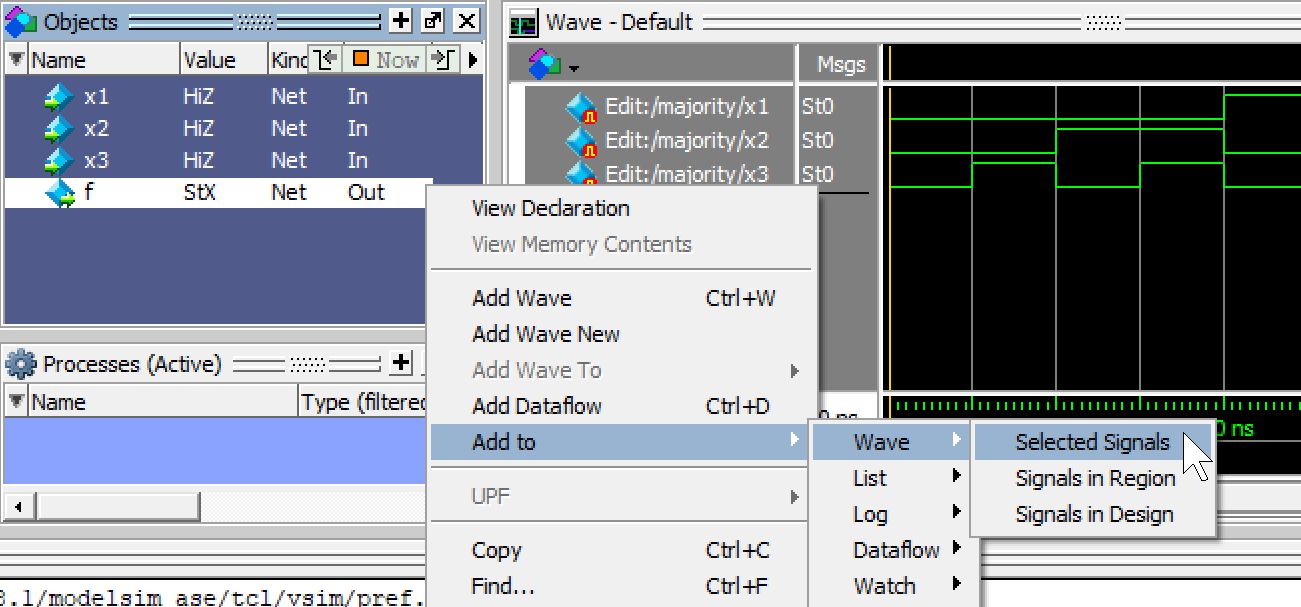
\includegraphics[scale=0.75]{figures/add_selected.png}
       \caption{Adding a signal to the \texttt{Wave} window.} 
	 \label{fig:22}
	 \end{center}
\end{figure}

\begin{figure}[H]
   \begin{center}
      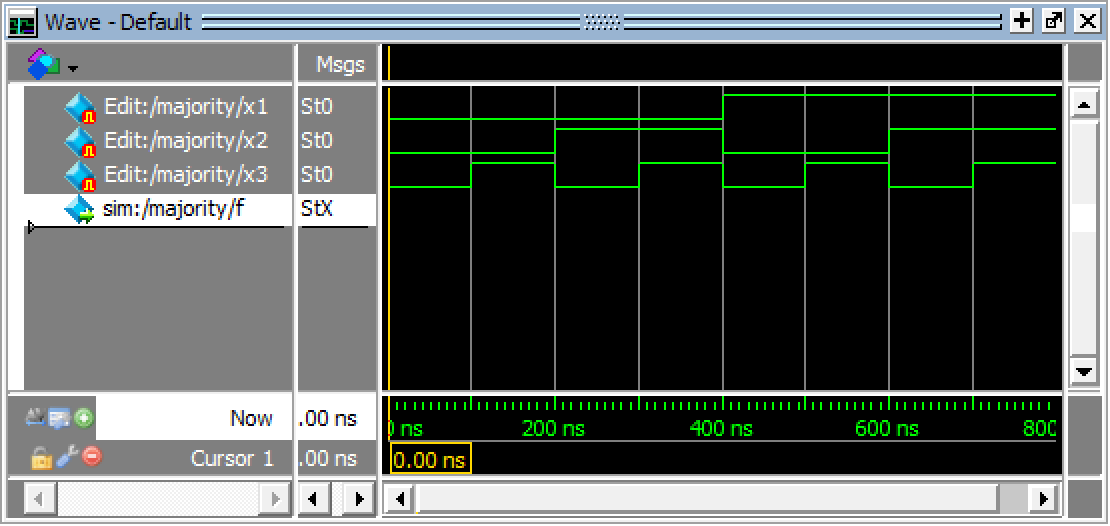
\includegraphics[scale=0.75]{figures/complete_wave.png}
       \caption{The completed \texttt{Wave} window.} 
	 \label{fig:23}
	 \end{center}
\end{figure}

Save the created waveforms by going to {\sf File > Save Format} in the \texttt{Wave} window. 
We will save the file using the default name {\it wave.do}, as indicated in Figure~\ref{fig:24}.

\begin{figure}[H]
   \begin{center}
      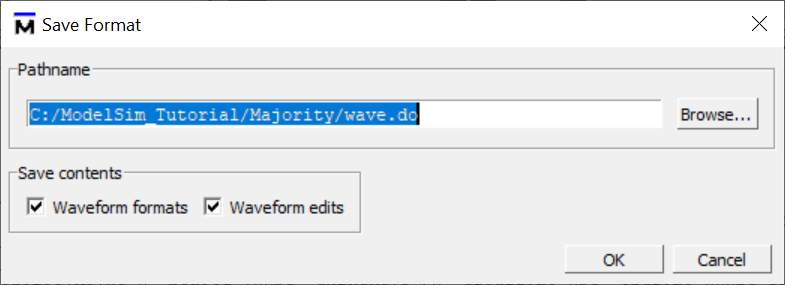
\includegraphics[scale=1.0]{figures/figure24.png}
   \caption{Saving the waveform file.} 
	 \label{fig:24}
	 \end{center}
\end{figure}

\section{Simulation}

To perform the simulation, in the toolbar area of the ModelSim GUI specify that the simulation 
should run for 800~ns, as illustrated in Figure~\ref{fig:26} (If you don't see this toolbar, 
right-click in the toolbar area and select {\sf Simulate}). Then, click on the
{\sf Run} icon, as indicated in Figure~\ref{fig:26}. The result of the simulation will be 
displayed as presented in the figure. Observe that the output {\it f} is equal to 1 whenever 
two or three inputs have the value 1, which verifies the correctness of our design.

\begin{figure}[H]
   \begin{center}
      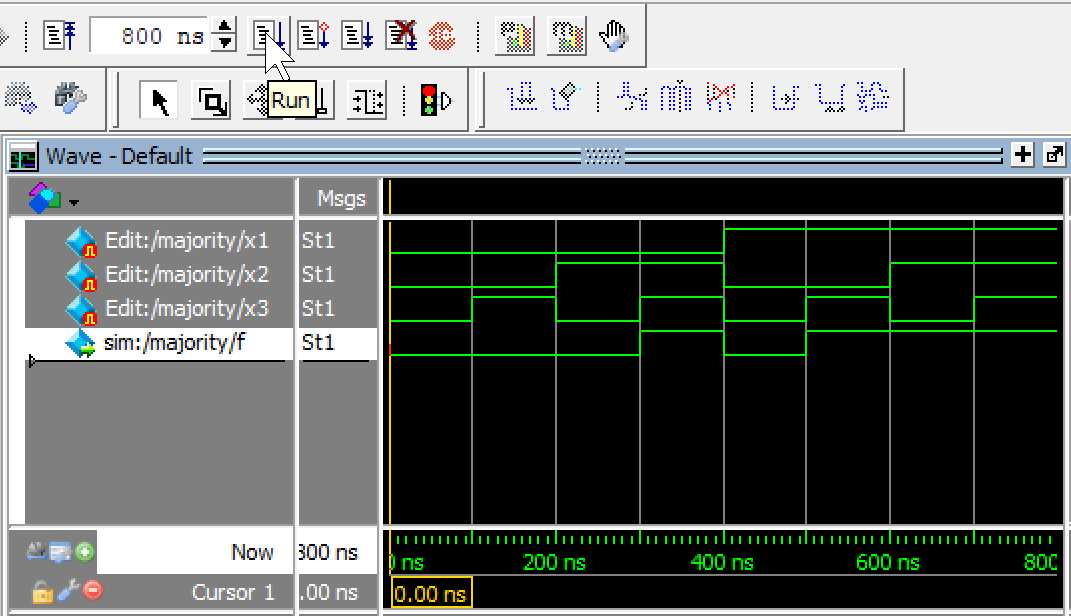
\includegraphics[scale=0.75]{figures/sim_run.png}
   \caption{Running the simulation.} 
	 \label{fig:26}
	 \end{center}
\end{figure}

\section{Making Changes and Resimulating}

Changes in the input waveforms can be made using the approaches explained above. Then, it
is necessary to restart the simulation using the altered waveforms. For example, change the
waveform for $x_1$ to have the logic value 1 in the interval from 0 to 200 ns, as indicated
in Figure~\ref{fig:28}. Now, click on the {\sf Restart} icon shown in the figure. A pop-up box in
Figure~\ref{fig:29} will appear. Leave the default entries and click {\sf OK}. Upon returning 
to the \texttt{Wave} window, simulate the design again by clicking on the {\sf Run} icon. 
The result is given in Figure~\ref{fig:30}.

\begin{figure}[H]
   \begin{center}
      
\includegraphics[scale=1.0]{figures/figure28.png}
   \caption{Changed input waveforms.} 
	 \label{fig:28}
	 \end{center}
\end{figure}

\begin{figure}[H]
   \begin{center}
      
\includegraphics[scale=0.8]{figures/figure29.png}
   \caption{The Restart box.} 
	 \label{fig:29}
	 \end{center}
\end{figure}

\begin{figure}[H]
   \begin{center}
      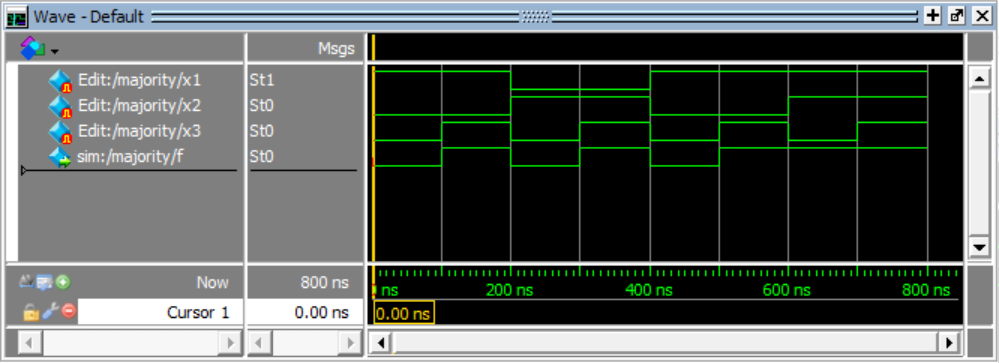
\includegraphics[scale=1.0]{figures/figure30.png}
   \caption{Result of the new simulation.} 
	 \label{fig:30}
	 \end{center}
\end{figure}

\noindent
Simulation is a continuous process. It can be stopped by selecting 
{\sf Simulate $>$ End Simulation} in the main ModelSim window.

\newpage
\section{Simulating a Circuit without Drawing Waveforms}

We will use another ModelSim project to illustrate some additional features
of the \texttt{Wave} window.  Consider the circuit given in Figure~\ref{fig:mux_4bit}, 
which is a 2-to-1 multiplexer for four-bit values. Part $a$ of the figure shows how the
circuit is constructed using 2-to-1 multiplexers, and Figure~\ref{fig:mux_4bit}$b$ gives 
the circuit symbol.  If the input $s = 0$ then the four-bit output $M = X$, 
else if $s = 1$ then $M = Y$. 

\begin{figure}[H]
   \begin{center}
      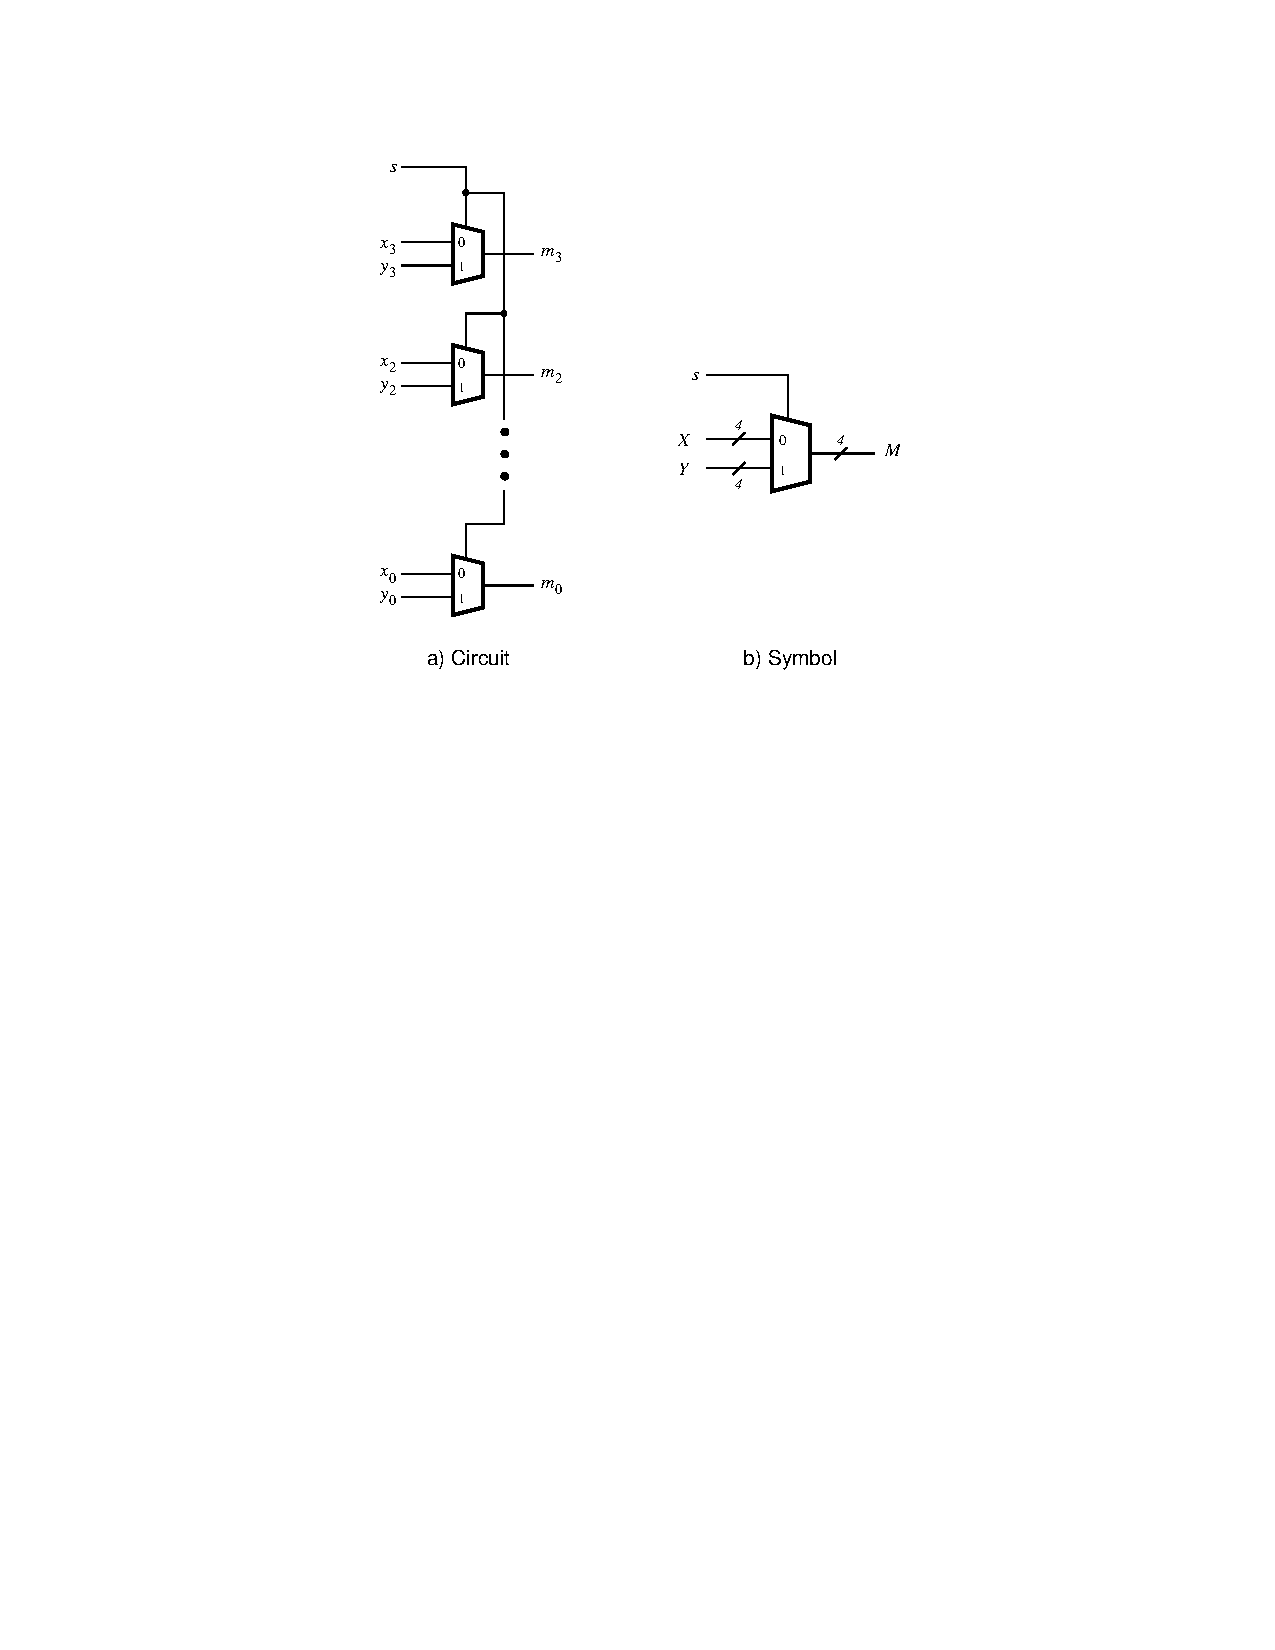
\includegraphics[scale=1.0]{figures/mux_4bit.pdf}
   \caption{A 2-to-1 multiplexer for four-bit values.} 
	 \label{fig:mux_4bit}
	 \end{center}
\end{figure}

This multiplexer circuit can be specified by using the Verilog code shown below.
~\\
\begin{lstlisting}[language=Verilog]
module Mux_4bit (X, Y, s, M);
    input [3:0] X, Y;        // input data
    input s;                 // select signal
    output [3:0] M;          // output data

    assign M[0] = (~s & X[0]) | (s & Y[0]);
    assign M[1] = (~s & X[1]) | (s & Y[1]);
    assign M[2] = (~s & X[2]) | (s & Y[2]);
    assign M[3] = (~s & X[3]) | (s & Y[3]);
endmodule
\end{lstlisting}

In the folder named {\it ModelSim\_Tutorial} that you created for this tutorial, make a new
subfolder called {\it Mux\_4bit} to hold the ModelSim files for this project.
In the folder {\it ModelSim\_Tutorial$\backslash$Mux\_4bit} enter the Verilog code for 
the multiplexer circuit into a file called {\it Mux\_4bit.v}.

In ModelSim, make a new project by selecting {\sf File $>$ New $>$ Project}, which opens the window 
from Figure~\ref{fig:1} (if ModelSim prompts you to close the currently-open project, 
select {\sf Yes}).  In the \texttt{Create Project} pop-up box from Figure~\ref{fig:2} give 
the project the name {\sf Mux\_4bit} and use the {\sf Browse} button to set the 
\texttt{Project Location} to {\it ModelSim\_Tutorial$\backslash$Mux\_4bit}. 
Click {\sf OK} to reach the pop-up from Figure~\ref{fig:3} and then select 
{\sf Add Existing File}. In the window from Figure~\ref{fig:4} use the {\sf Browse} button 
to add your {\it Mux\_4bit.v} file to the project. 

Now, in the window from Figure~\ref{fig:6} select the {\sf Compile $>$ Compile All} command.
If you typed the Verilog code for the multiplexer correctly, then you should see a message in the
\texttt{Transcript} window reporting compilation success. If there are any errors, then fix 
the code and compile again.

\section{Specifying Simulation Inputs}

To perform simulation of the multiplexer, select the command {\sf Simulate $>$ Start Simulation}
to reach the window in Figure~\ref{fig:mux_start_sim}. As indicated in the figure, expand the 
{\sf work} folder, click on the {\sf Mux\_4bit} design, and then select {\sf OK}. Your ModelSim
display should now look like the one shown in Figure~\ref{fig:mux_main}. To populate the 
\texttt{Wave} window as displayed in the figure, first click on the signal {\sf X} in the 
\texttt{Objects} window and then shift-click on the signal {\sf M} so that all signals are selected.
Now, drag-and-drop the selected signals into the \texttt{Wave} window. Set the {\sf Zoom Range} 
of the Wave window to 80~ns.
~\\

\begin{figure}[H]
   \begin{center}
      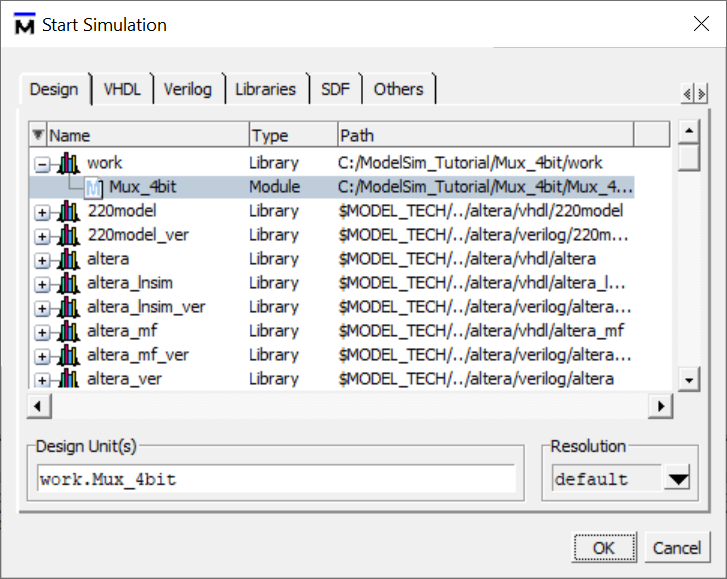
\includegraphics[scale=0.70]{figures/mux_start_sim.png}
   \caption{The start simulation window.} 
	 \label{fig:mux_start_sim}
	 \end{center}
\end{figure}

\begin{figure}[H]
   \begin{center}
      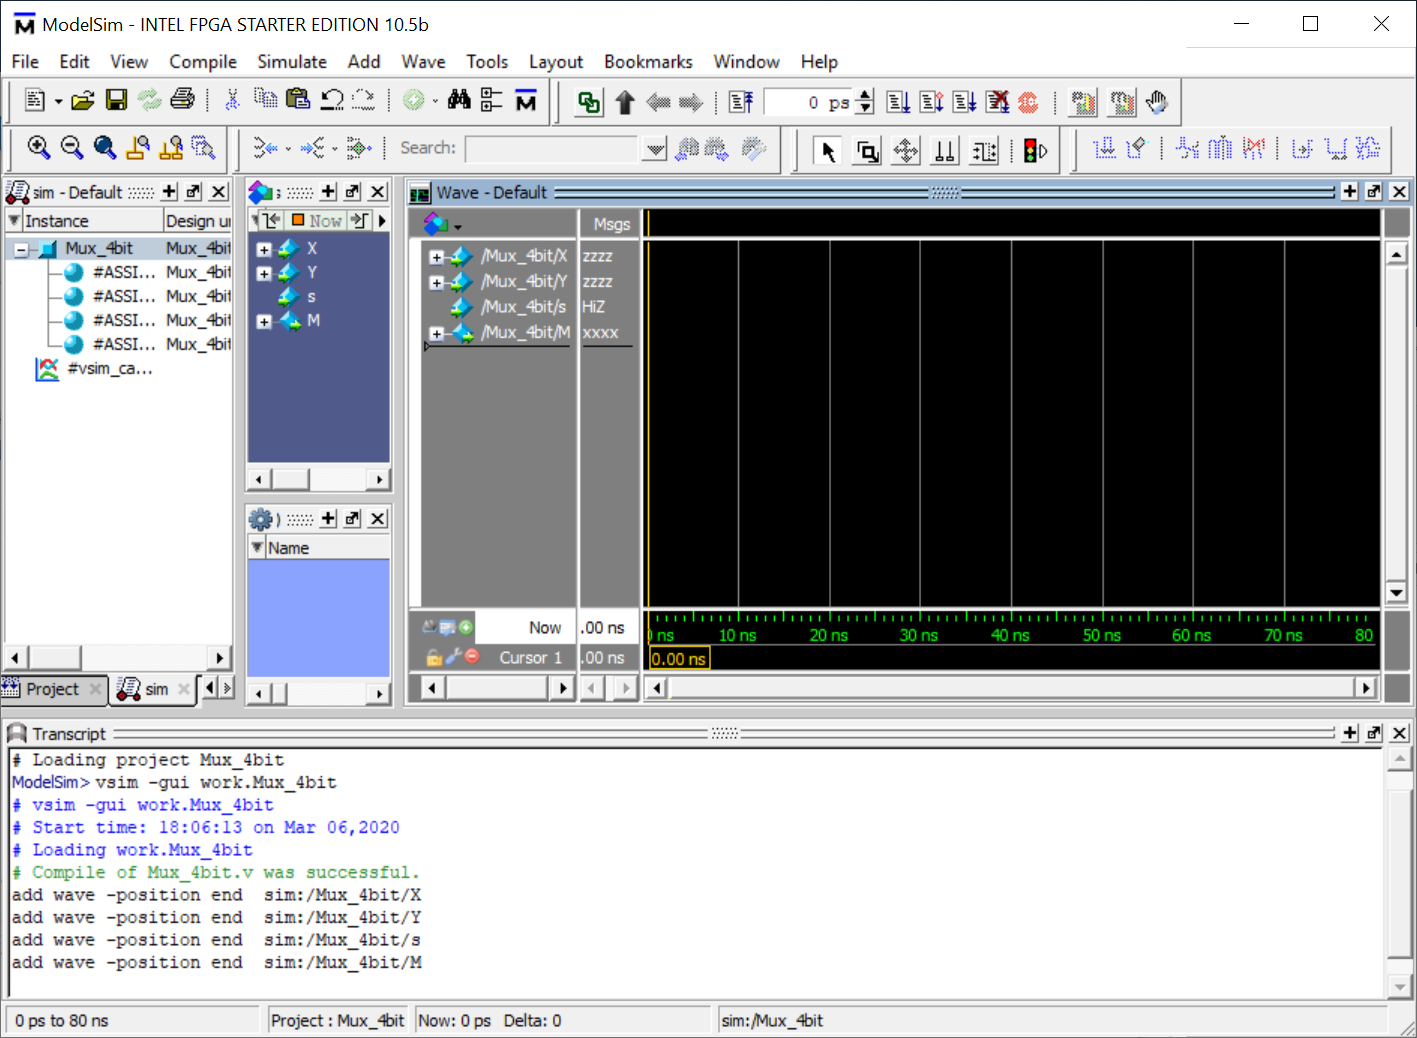
\includegraphics[width=.95\textwidth]{figures/mux_main.png}
   \caption{The ModelSim window for simulation of the multiplexer.} 
	 \label{fig:mux_main}
	 \end{center}
\end{figure}

Before beginning the simulation we will first illustrate how the \texttt{Wave} window
can be used to select a specific number-radix for displaying the value of a signal. 
Right-click on the name of the signal {\sf X} in the \texttt{Wave} window, as illustrated 
in Figure~\ref{fig:mux_radix}, and note that several radix choices are available. In this 
case select {\it Radix > Binary}. Use this same procedure to set the radices for the other
signals to {\sf Binary}, or to some other choice if you prefer.

\begin{figure}[H]
   \begin{center}
      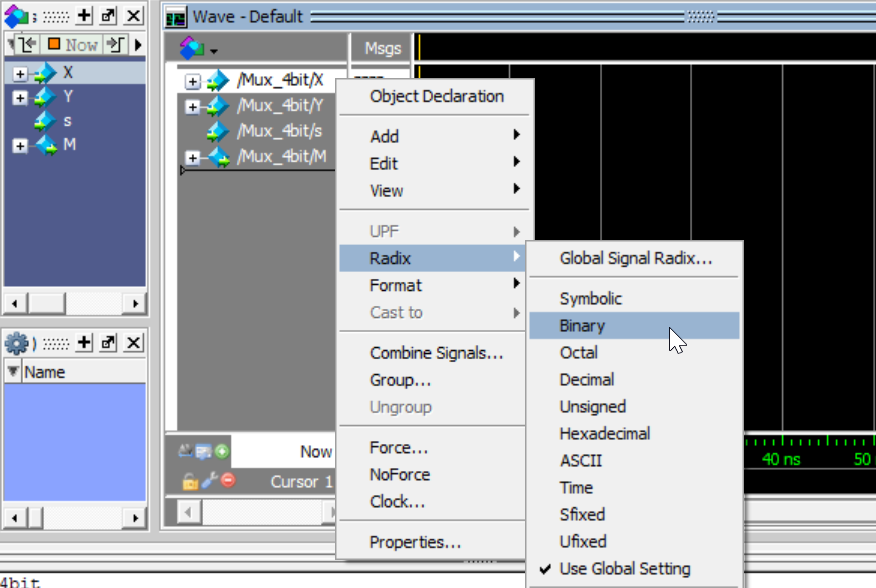
\includegraphics[scale=.75]{figures/mux_radix.png}
   \caption{Setting a waveform radix.} 
	 \label{fig:mux_radix}
	 \end{center}
\end{figure}

For the previous ModelSim project described in this tutorial we employed features of the 
\texttt{Wave} window to {\it draw} waveforms that were used as inputs to the simulation. 
For this project we will use a different method by {\it forcing} the values of signals. 
Right-click on the {\it X} signal, as illustrated in Figure~\ref{fig:mux_force}, and 
select {\sf Force}. This action opens the pop-up window in Figure~\ref{fig:mux_force_5} that 
displays the signal name $X$ and allows its value to be set.  As illustrated in
the figure set the $X$ signal to the binary value \texttt{0101}.

\begin{figure}[H]
   \begin{center}
      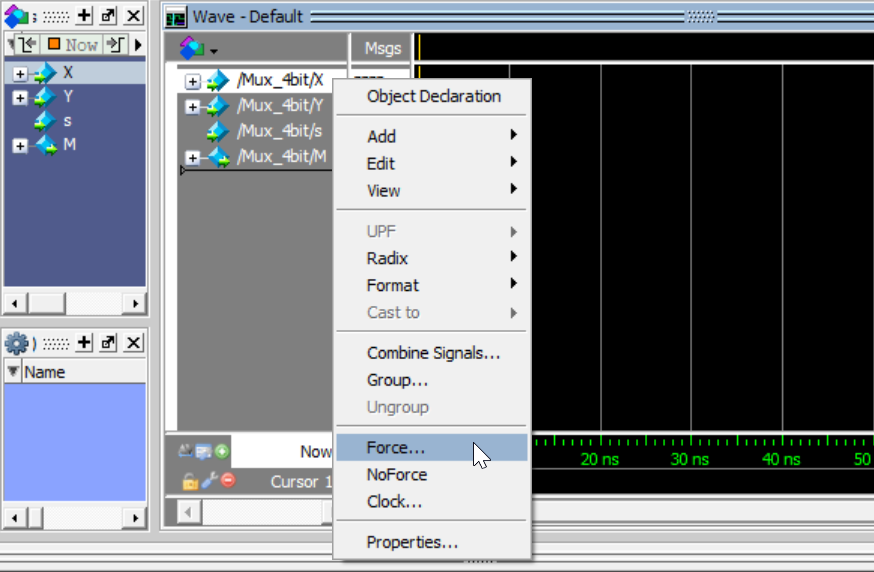
\includegraphics[scale=.75]{figures/mux_force.png}
       \caption{Selecting the {\sf Force} command.} 
	 \label{fig:mux_force}
	 \end{center}
\end{figure}

\begin{figure}[H]
   \begin{center}
      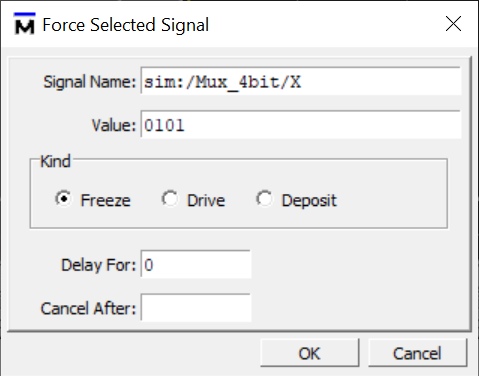
\includegraphics[scale=.75]{figures/mux_force_5.png}
       \caption{Forcing the {\it X} signal to the value 0101.} 
	 \label{fig:mux_force_5}
	 \end{center}
\end{figure}

Next right-click on the {\it Y} signal and use the \texttt{Force} command to set it to the
binary value 1010. Finally, use the \texttt{Force} command to set the {\it s} signal to
the value 0 so that the multiplexer selects input $X$. 
Now that the input values have been set, we can run the simulation for an
initial time period, such as 20 ns. To run the simulation for 20~ns you can use the \texttt{Run
Length} toolbar box from Figure~\ref{fig:26}. Alternatively you can enter the command 
{\sf run 20 ns} in the \texttt{Transcript} window. Perform the simulation to get the result 
shown in Figure~\ref{fig:mux_20ns}.

\begin{figure}[H]
   \begin{center}
      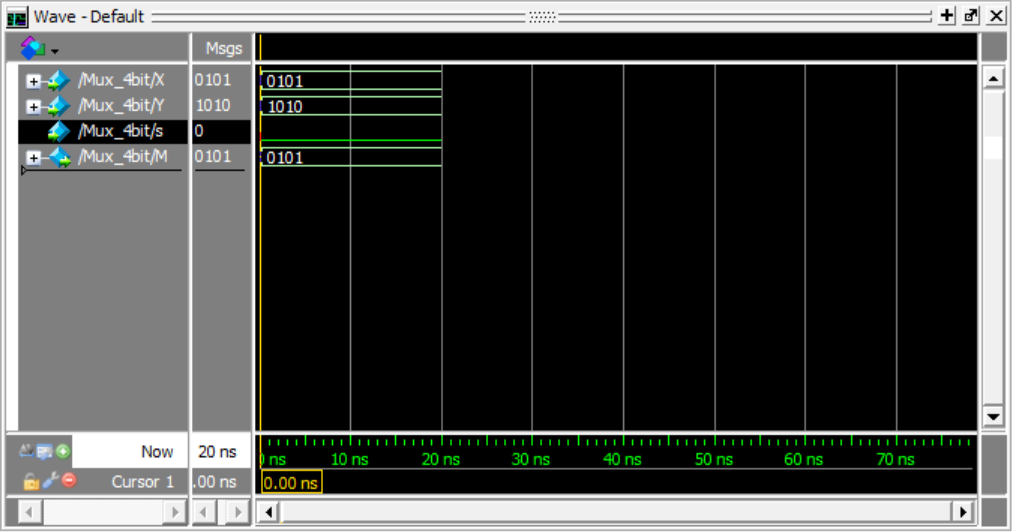
\includegraphics[scale=.75]{figures/mux_20ns.png}
       \caption{Waveforms after running the simulation for 20 ns.} 
	 \label{fig:mux_20ns}
	 \end{center}
\end{figure}

Now, right-click on the {\it s} signal again and select the {\sf Force} command. In the window 
from Figure~\ref{fig:mux_force_5} set the {\it s} signal to 1, so that the multiplexer
selects input $Y$.
Then run the simulation for another 20~ns by using either the \texttt{Run Length} toolbar box
or by typing {\sf run 20 ns} in the \texttt{Transcript} window. Continue changing the
input values and running additional simulation time periods as desired. Example waveforms for
an 80 ns simulation are shown in Figure~\ref{fig:mux_80ns}.

\begin{figure}[H]
   \begin{center}
      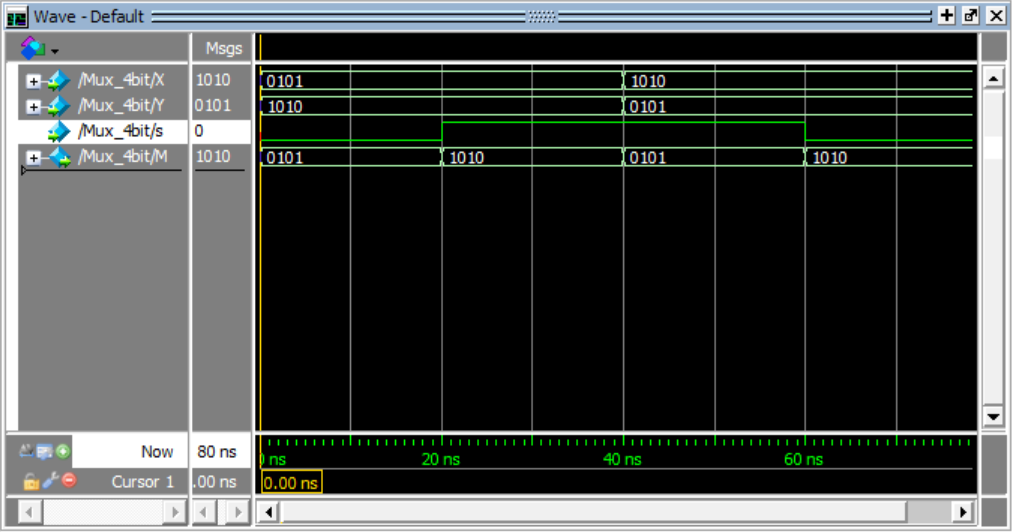
\includegraphics[scale=.75]{figures/mux_80ns.png}
       \caption{Waveforms after running the simulation.} 
	 \label{fig:mux_80ns}
	 \end{center}
\end{figure}

\section{Simulating a Sequential Circuit}

We will use another ModelSim project to illustrate some additional features
of the \texttt{Wave} window.  Consider the Verilog code shown below, which 
specifies a loadable down-counter:
~\\
\begin{lstlisting}[language=Verilog]
module counter (L, Clock, Data, Q);
    input L, Clock;
    input [2:0] Data;
    output reg [2:0] Q;

    wire E; 

    always @(posedge Clock)
        if (!L)
            Q <= Data;
        else if (E)
            Q <= Q - 3'b1;

    assign E = (Q != 3'b0);
endmodule
\end{lstlisting}

The counter can be synchronously loaded from the {\it Data} input when when the load input
$L = 0$. When the count reaches zero the enable $E$ is set to 0 and this stops the counter. 

In the folder named {\it ModelSim\_Tutorial} that you created for this tutorial, make a new
subfolder called {\it Counter} to hold the ModelSim files for this project.
In the folder {\it ModelSim\_Tutorial$\backslash$Counter}
enter the Verilog code for the down-counter into a file called {\it counter.v}.

In ModelSim, make a new project by selecting {\sf File $>$ New $>$ Project}, which opens the window 
from Figure~\ref{fig:1} (if ModelSim prompts you to close the currently-open project, select {\sf Yes}). 
In the \texttt{Create Project} pop-up box from Figure~\ref{fig:2} give the project the name 
{\sf counter} and use the {\sf Browse} button to set the \texttt{Project Location} to
{\it ModelSim\_Tutorial$\backslash$Counter}. Click {\sf OK} to reach the pop-up from 
Figure~\ref{fig:3} and then select {\sf Add Existing File}. In the window from 
Figure~\ref{fig:4} use the {\sf Browse} button to add your {\it counter.v} file to the project. 

Now, in the window from Figure~\ref{fig:6} select the {\sf Compile $>$ Compile All} command.
If you typed the Verilog code for the counter correctly, then you should see a message in the
\texttt{Transcript} window reporting compilation success. If there are any errors, then fix the code
and compile again.

\section{Specifying Simulation Inputs}

To perform simulation of the counter, select the command {\sf Simulate $>$ Start Simulation} to reach
the window in Figure~\ref{fig:counter_start_sim}. As indicated in the figure, expand the {\sf work} 
folder, click on the {\sf counter} design, and then select {\sf OK}. Your ModelSim display should
now look like the one shown in Figure~\ref{fig:counter_main}. To populate the 
\texttt{Wave} window as displayed in the figure, first click on the signal {\sf L} in the 
\texttt{Objects} window and then shift-click on the signal {\sf E} so that all signals are selected.
Now, drag-and-drop the selected signals into the \texttt{Wave} window. Set the {\sf Zoom Range} of the Wave
window to 1800~ns.

\begin{figure}[H]
   \begin{center}
      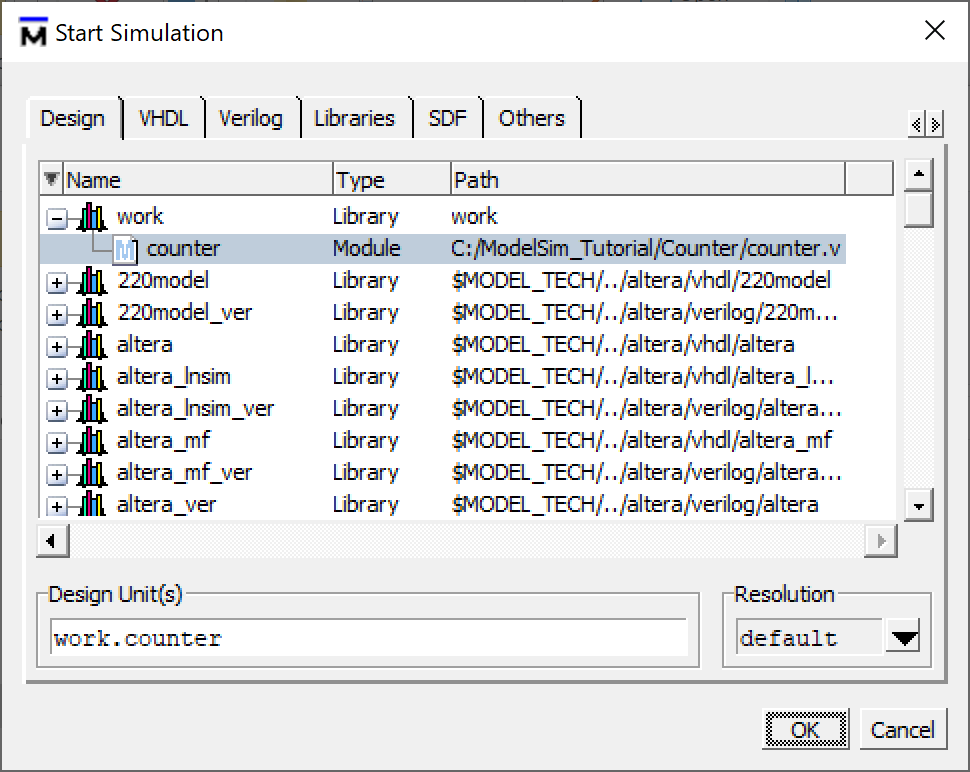
\includegraphics[scale=0.70]{figures/counter_start_sim.png}
   \caption{The start simulation window.} 
	 \label{fig:counter_start_sim}
	 \end{center}
\end{figure}

\begin{figure}[H]
   \begin{center}
      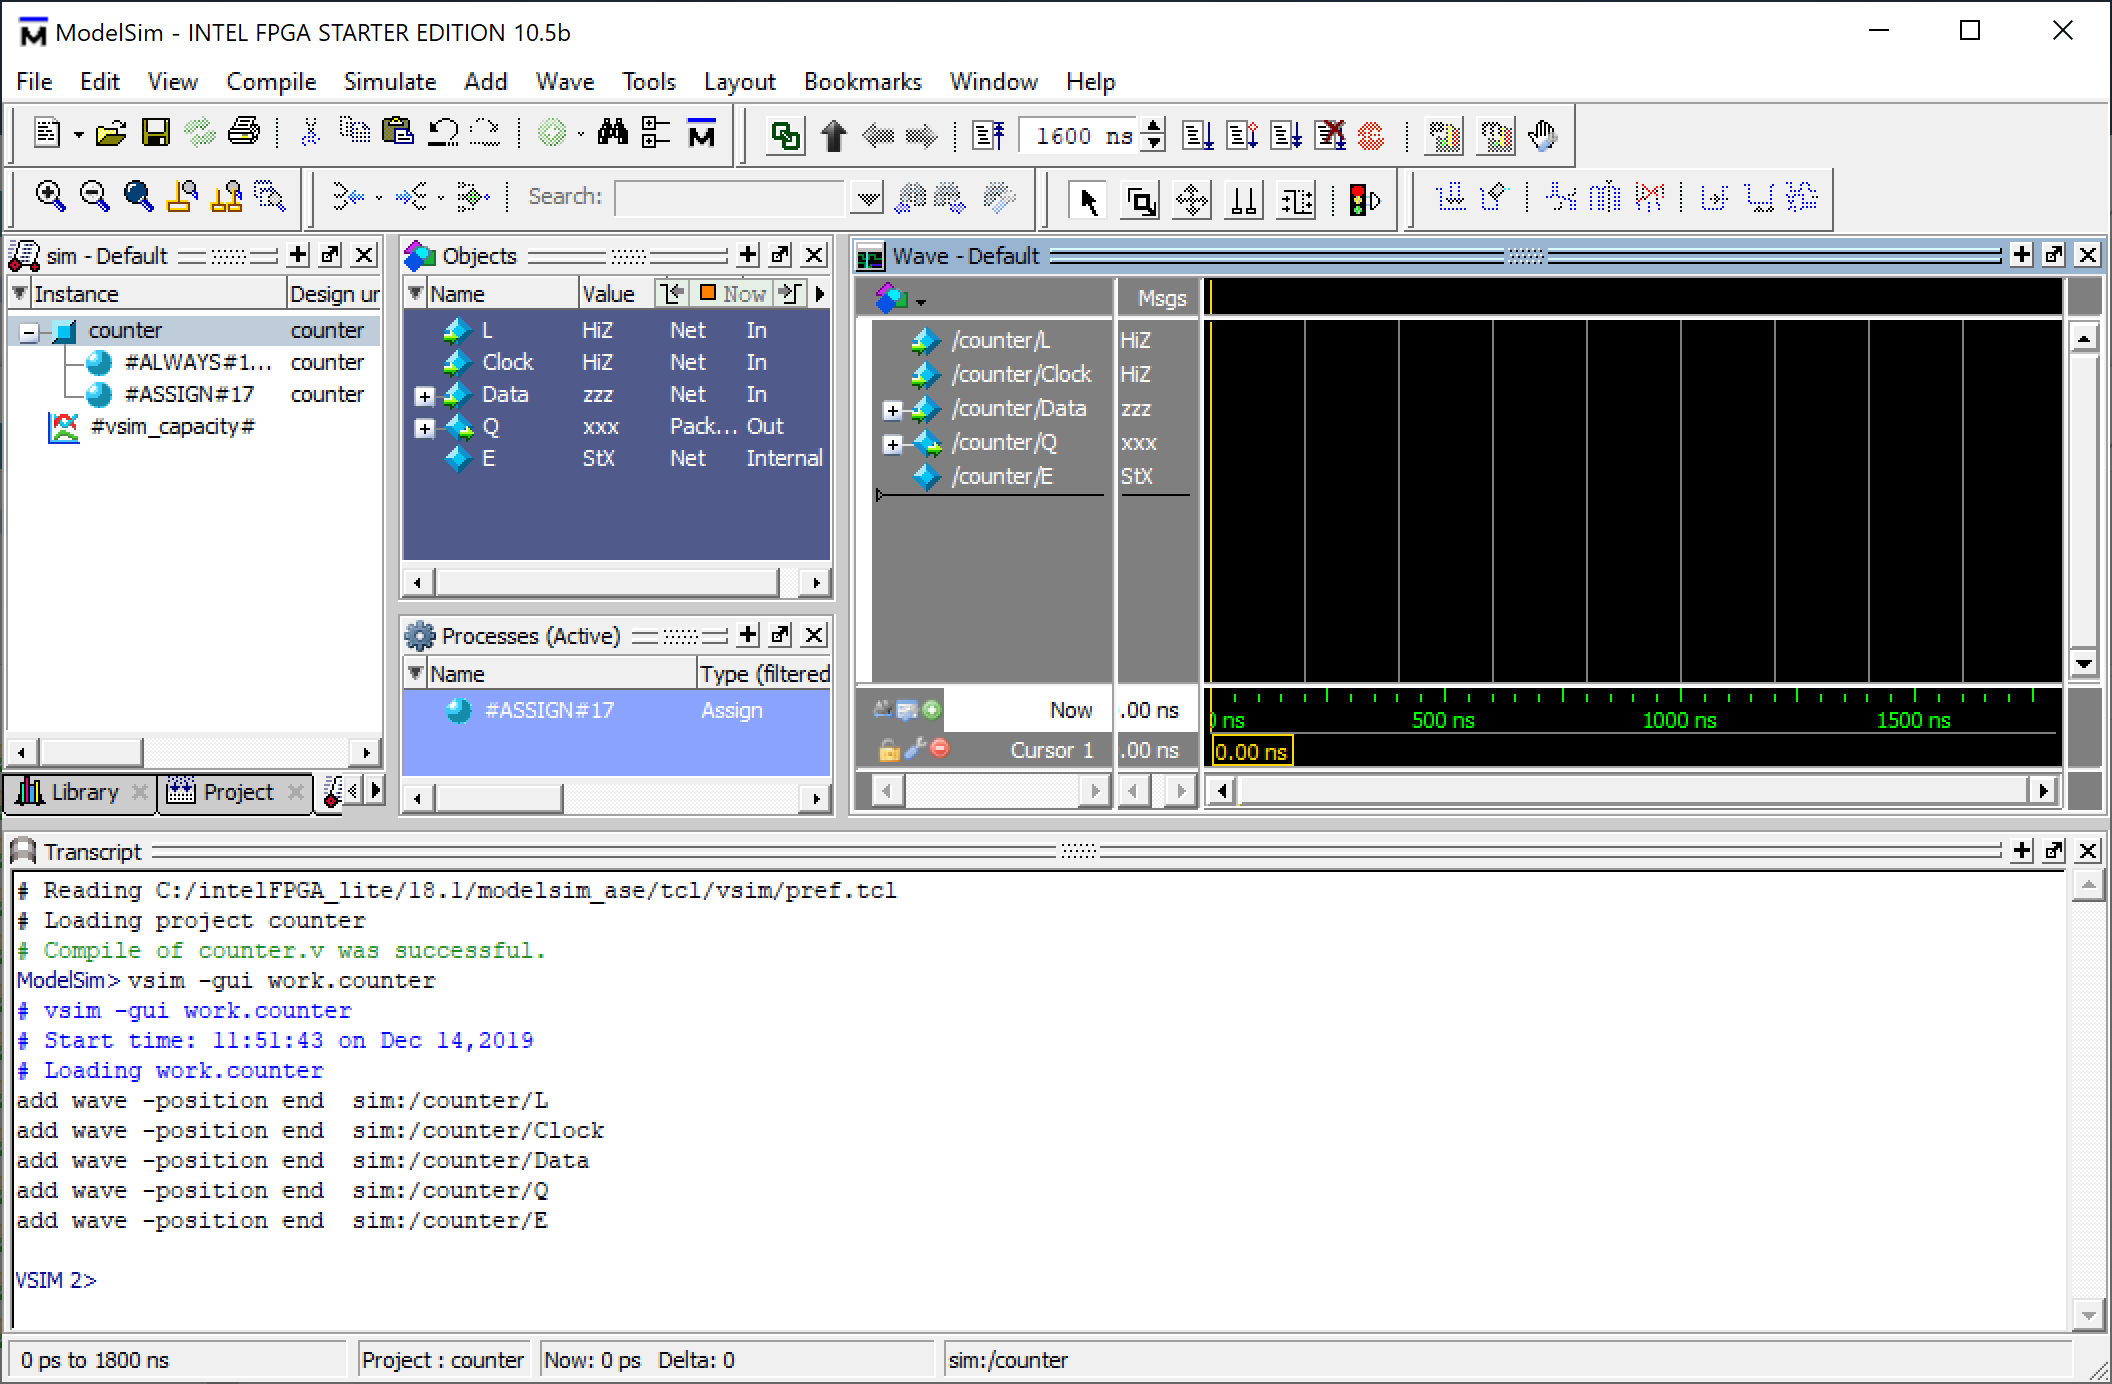
\includegraphics[width=.95\textwidth]{figures/counter_main.png}
   \caption{The ModelSim window for simulation of the counter.} 
	 \label{fig:counter_main}
	 \end{center}
\end{figure}

Before beginning the simulation we will illustrate some useful features of the \texttt{Wave} window.
For each signal we will first select a specific number-radix for displaying its value, and 
then assign the signal a customized display name. Right-click on the name of the 
signal {\sf L} in the \texttt{Wave} 
window, as illustrated in Figure~\ref{fig:counter_radix}, and select {\it Radix > Binary}. Use 
this same procedure to set the radix for {\sf Clock} to {\sf Binary}, {\sf Data} and {\sf Q}
to {\sf Unsigned}, and {\sf E} to {\sf Binary}.

\begin{figure}[H]
   \begin{center}
      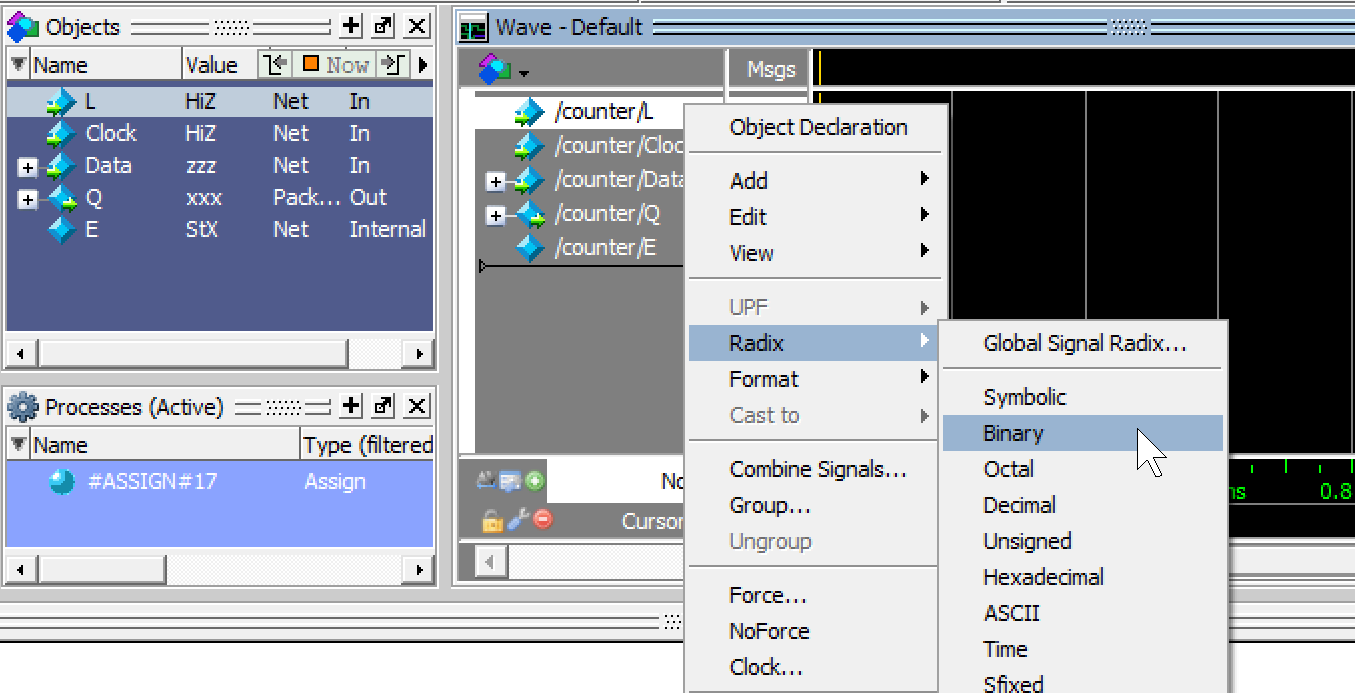
\includegraphics[scale=.75]{figures/counter_radix.png}
   \caption{Setting a waveform radix.} 
	 \label{fig:counter_radix}
	 \end{center}
\end{figure}

Now, as shown in Figure~\ref{fig:counter_prop}, right-click again on {\sf L} and select 
{\sf Properties} to open the dialog in Figure~\ref{fig:counter_name}. Set the {\sf Display Name}
to {\sf Load}. Then, use the same process to set the other display names as given in 
Figure~\ref{fig:counter_names}.

\begin{figure}[H]
   \begin{center}
      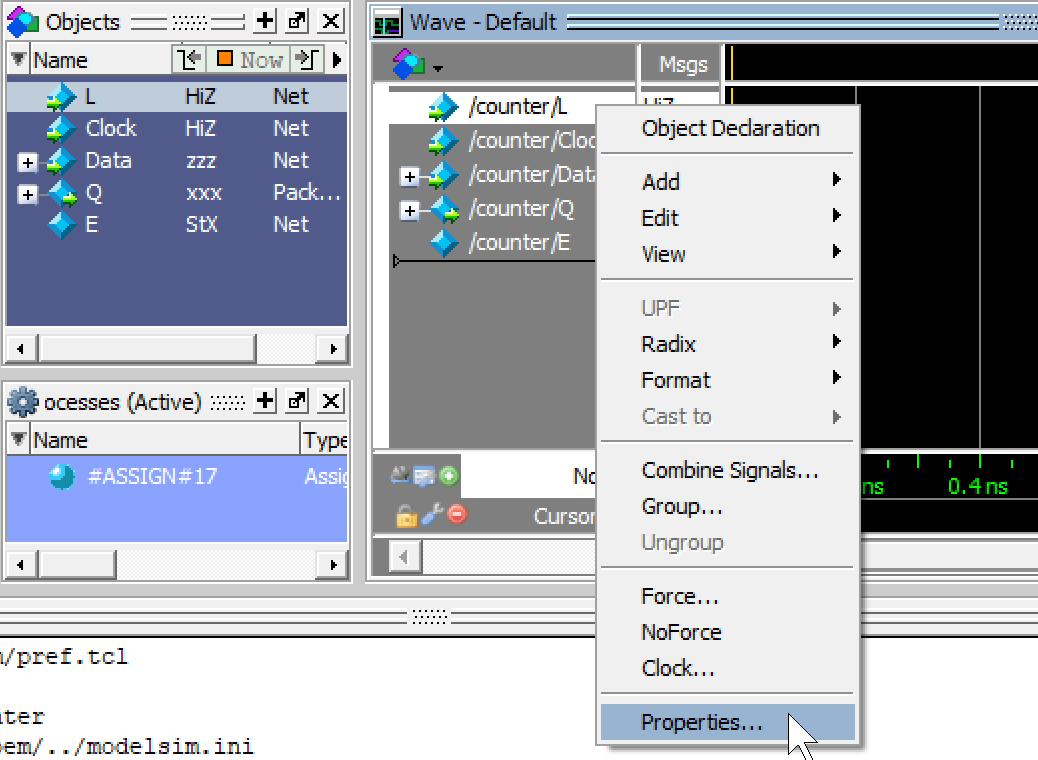
\includegraphics[scale=.75]{figures/counter_prop.png}
   \caption{The Properties dialog.} 
	 \label{fig:counter_prop}
	 \end{center}
\end{figure}

\begin{figure}[H]
   \begin{center}
      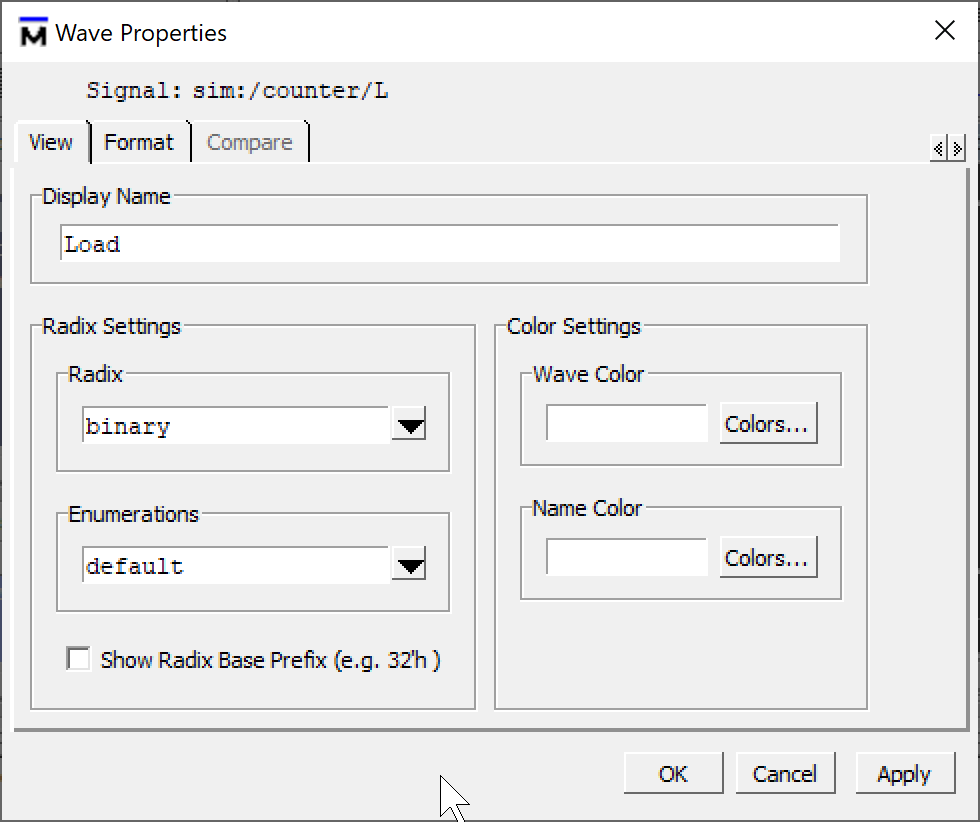
\includegraphics[scale=.75]{figures/counter_name.png}
   \caption{Setting a display name.} 
	 \label{fig:counter_name}
	 \end{center}
\end{figure}

\begin{figure}[H]
   \begin{center}
      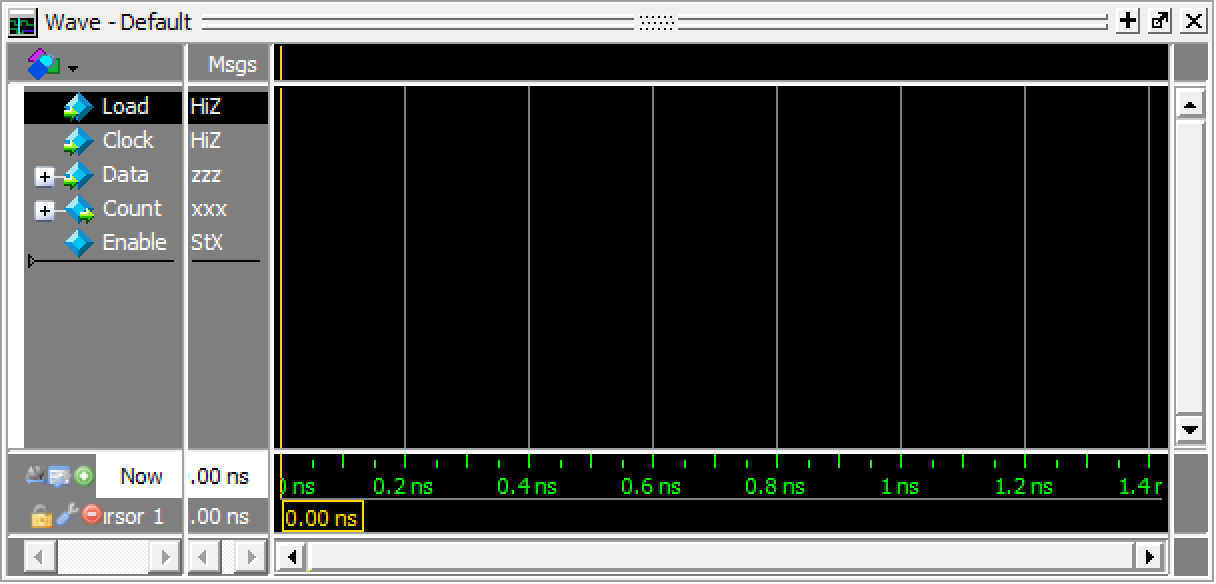
\includegraphics[scale=.75]{figures/counter_names.png}
   \caption{The renamed signals.} 
	 \label{fig:counter_names}
	 \end{center}
\end{figure}

For the previous ModelSim project described in this tutorial we employed features of the 
\texttt{Wave} window to {\it draw} waveforms that were used as inputs to the simulation. For 
this project we will use a different method by {\it forcing} the values of signals. Right-click
on the {\it Load} signal, as illustrated in Figure~\ref{fig:counter_force}, and select 
{\sf Force}. This action opens the pop-up window in Figure~\ref{fig:counter_force_0} that 
displays the original signal name $L$ and allows its value to be set. As illustrated in
the figure set the $L$ signal to the value 0.

\begin{figure}[H]
   \begin{center}
      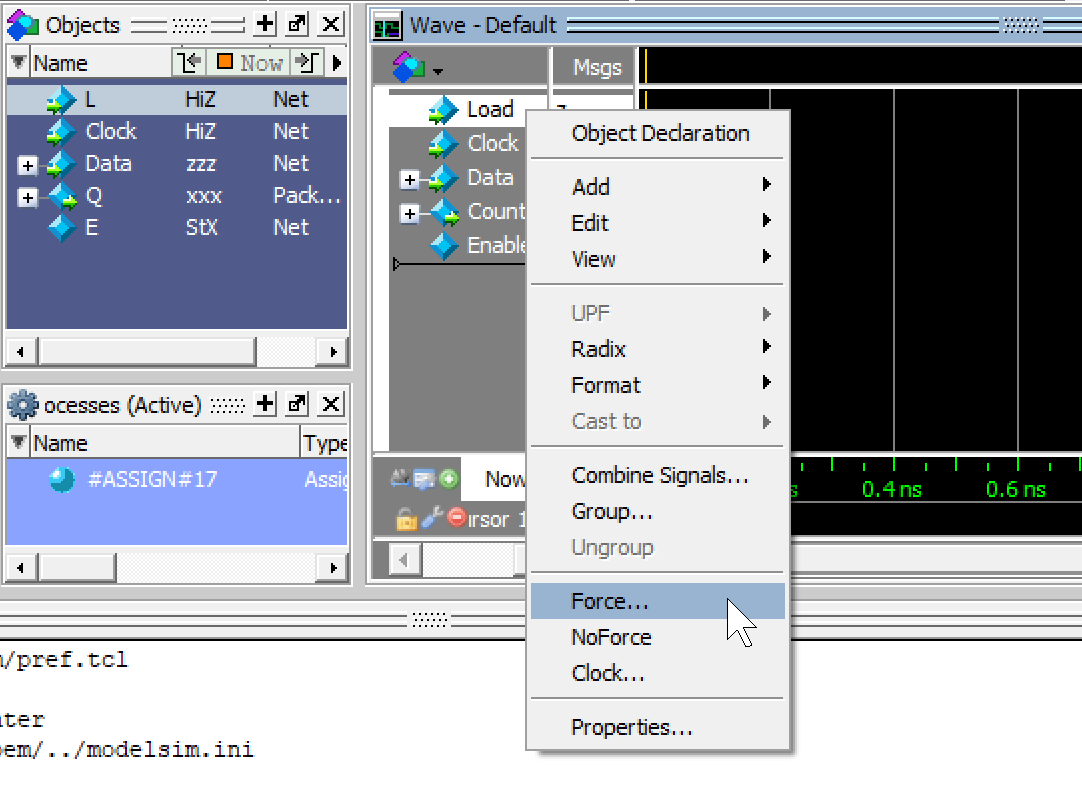
\includegraphics[scale=.75]{figures/counter_force.png}
       \caption{Selecting the {\sf Force} command.} 
	 \label{fig:counter_force}
	 \end{center}
\end{figure}

\begin{figure}[H]
   \begin{center}
      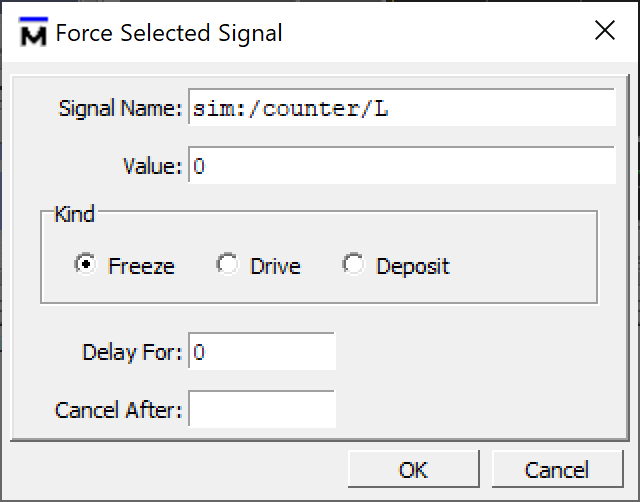
\includegraphics[scale=.75]{figures/counter_force_0.png}
       \caption{Forcing the {\it Load} signal to the value 0.} 
	 \label{fig:counter_force_0}
	 \end{center}
\end{figure}

Next, in the \texttt{Wave} window right-click on the {\it Clock} signal and select the 
\texttt{Clock} command to open the pop-up in Figure~\ref{fig:counter_clock_200}. In the {\sf Period} box
specify a clock-period of 200~ns, as illustrated in the figure, and then click {\sf OK}. Finally, set the
value of the {\it Data} input signal by right-clicking on its waveform and selecting the {\it Force} command.
As depicted in Figure~\ref{fig:counter_force_6} specify a data value of 10\#6. This syntax means that a number
base of 10 is being used to specify a signal value of 6.

\begin{figure}[H]
   \begin{center}
      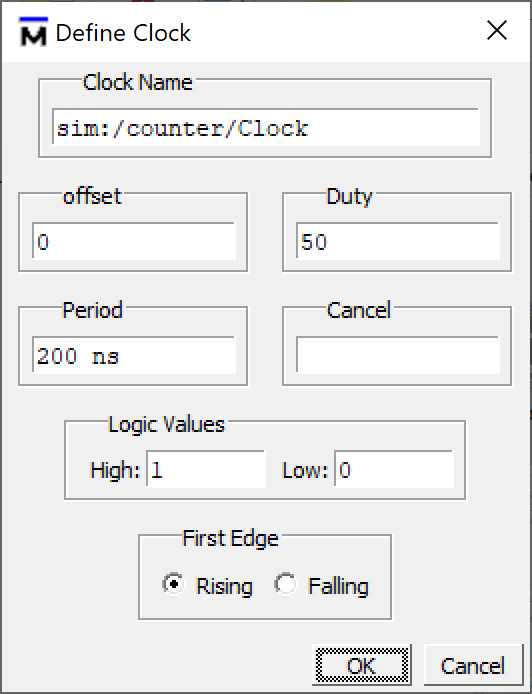
\includegraphics[scale=.75]{figures/counter_clock_200.png}
       \caption{Setting the {\it Clock} period to 200 ns.} 
	 \label{fig:counter_clock_200}
	 \end{center}
\end{figure}

\begin{figure}[H]
   \begin{center}
      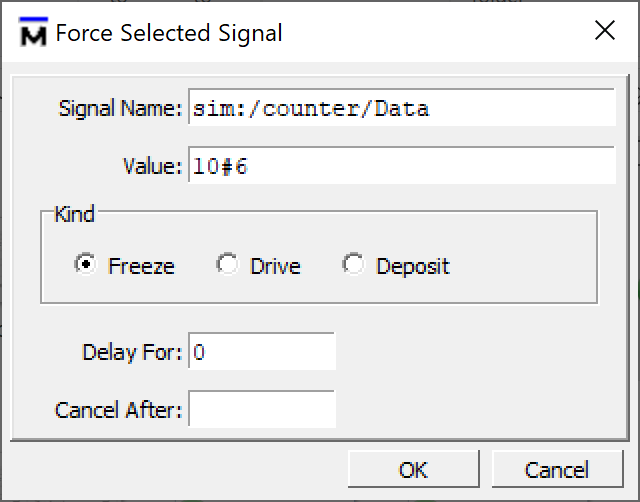
\includegraphics[scale=.75]{figures/counter_force_6.png}
       \caption{Forcing the value of the {\it Data} signal..} 
	 \label{fig:counter_force_6}
	 \end{center}
\end{figure}

Since the {\it Load} signal is asserted to 0 we can now initialize the counter from the {\it Data} input 
by running the circuit for one clock cycle. To run the simulation for 200~ns you can use the \texttt{Run
Length} toolbar box from Figure~\ref{fig:26}. Alternatively you can enter the command {\sf run 200 ns} in the
\texttt{Transcript} window. Perform the simulation to get the result shown in Figure~\ref{fig:counter_200ns}.

Now, right-click on the {\it Load} signal again and select the {\sf Force} command. In the window from 
Figure~\ref{fig:counter_force_0} set the {\it Load} signal to 1, so that it is no longer asserted. 
Finally, run the simulation for another 1600~ns by using either the \texttt{Run Length} toolbar box
or by typing {\sf run 1600 ns} in the \texttt{Transcript} window. As shown in 
Figure~\ref{fig:counter_1600ns} the counter decrements on each active clock edge until it reaches 0, after
which {\it Enable = 0} and the counter is stopped. 

\begin{figure}[H]
   \begin{center}
      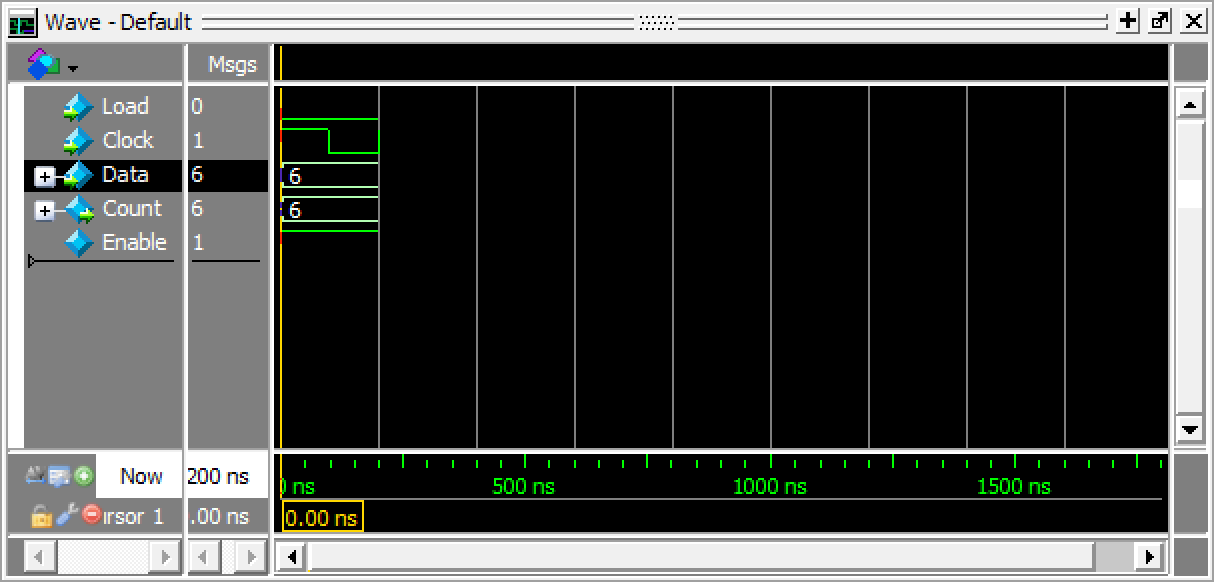
\includegraphics[scale=.75]{figures/counter_200ns.png}
       \caption{Waveforms after running the simulation for 200 ns.} 
	 \label{fig:counter_200ns}
	 \end{center}
\end{figure}

\begin{figure}[H]
   \begin{center}
      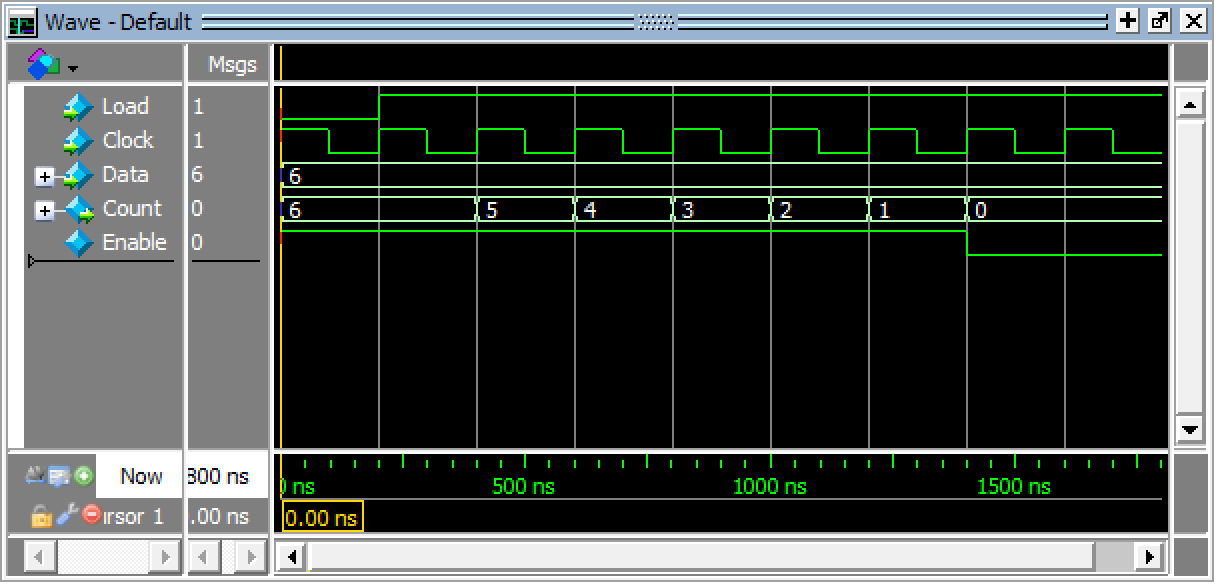
\includegraphics[scale=.75]{figures/counter_1600ns.png}
       \caption{Waveforms after running the full simulation.} 
	 \label{fig:counter_1600ns}
	 \end{center}
\end{figure}

You can select the {\it File > Save Format} command to save the formatting information for the waveforms,
using a filename such as {\it wave.do}. If you quit ModelSim and then later reload the {\it counter} project,
then the waveform formats can be reloaded by first starting a new simulation and then entering the command 
{\sf do wave.do} in the \texttt{Transcript} window.

\section{Concluding Remarks}

The purpose of this tutorial is to provide a quick introduction to ModelSim, explaining only
the rudimentary aspects of functional simulation that can be performed using the ModelSim
Graphical User Interface. More details about the ModelSim simulator can be found in other 
tutorials that are available on the internet.

% Copyright

%\newcommand{\datePublished}{Mar 2022}

\newcommand{\versnum}{21.1} %version number quartus/AMP
\newcommand{\quartusname}{Quartus\textsuperscript{\textregistered} Prime}	
\newcommand{\textBar}{For \quartusname{} \versnum{}}
\newcommand{\thisyear}{2022 } %for copyright
\newcommand{\company}{FPGAcademy.org}
\newcommand{\longteamname}{FPGAcademy.org}
\newcommand{\teamname}{FPGAcademy}
\newcommand{\website}{FPGAcademy.org}

\newcommand{\productAcronym}{AMP}
\newcommand{\productNameShort}{Monitor Program}

\newcommand{\productNameMedTM}{Monitor Program}
\newcommand{\productNameMed}{Monitor Program}

%\newcommand{\headerLogoFilePath}[1]{#1/FPGAcademy.png}



%%%%%%%%%%%%%%%%%%%%%%%%%%%%%%%%%%%%%%%%
%%% FPGAcademy Copyright Information %%%
%%%%%%%%%%%%%%%%%%%%%%%%%%%%%%%%%%%%%%%%

%Always put the copyright on a new page (clear page), with some vertical space from top
\clearpage
\vspace{1in}

\noindent

Copyright {\copyright} FPGAcademy.org. All rights reserved. FPGAcademy and the FPGAcademy logo are trademarks of  FPGAcademy.org.  This document is being provided on an ``as-is'' basis and as an accommodation and therefore all warranties, representations or guarantees of any kind (whether express, implied or statutory) including, without limitation, warranties of merchantability, non-infringement, or fitness for a particular purpose, are specifically disclaimed.

%FPGAcademy assumes no responsibility or liability arising out of the application or use of any information,  product,  or  service  described  herein  except  as  expressly  agreed  to  in  writing  by  FPGAcademy.



**Other names and brands may be claimed as the property of others.




\end{document}
